\documentclass[12pt, b5paper, oldfontcommands]{memoir}
% Margins
\usepackage[b5paper,total={6in, 9in}]{geometry}
\geometry{margin=2.4cm, top=2.5cm}

% Citations at the end of each chapter
\usepackage[sectionbib,square,comma]{natbib}
\usepackage{chapterbib}
\bibliographystyle{bib/genbibstyle}

% Required for LaTeXDraw
%\usepackage[usenames,dvipsnames]{pstricks}
%\usepackage{pstricks-add}
%\usepackage{epsfig}
%\usepackage{pst-grad} % For gradients
%\usepackage{pst-plot} % For axes

% Switched to tikz ecosystem
\usepackage{forest}
\usepackage{graphicx}
%\usepackage{svg} % For \includesvg

\usepackage[space]{grffile} % For spaces in paths
\usepackage{etoolbox} % For spaces in paths
\makeatletter % For spaces in paths
\patchcmd\Gread@eps{\@inputcheck#1 }{\@inputcheck"#1"\relax}{}{}
\makeatother

% Required for grammar trees
\usepackage{pst-node,pst-tree}

%\usepackage{createspace}
%\usepackage{geometry}
%\usepackage{graphicx}
%\usepackage{tikz}

%\usepackage[utf8]{inputenc}
%\usepackage{fix-cm}

\usepackage{tgheros} % "TEX Gyre Heros", Helvetica, code: qhv
%\usepackage{tgbonum} % "TEX Gyre Bonum", ITCBookman, code: qbk
% Keep commented. Somehow ptm still loads, while uncommenting messes up Greek letters.
%\usepackage{mathptmx} % Times, code: ptm

\usepackage[utf8]{inputenc}
\usepackage[T1]{fontenc}
\usepackage[english]{babel}
\usepackage{anyfontsize}
%\usepackage{microtype}
\usepackage{sfmath} % Sans Serif math fonts
\renewcommand{\rmdefault}{ptm} % Times
\renewcommand{\sfdefault}{qhv} % Helvetica
\renewcommand{\familydefault}{\rmdefault}

\usepackage[fleqn]{amsmath}
\usepackage{mathrsfs} % Math script
\usepackage{mathtools}
%\usepackage{textgreek} % Greek characters in text mode.
%\newcommand{\tl}{λ}
\newcommand{\tlb}[1]{$\boldsymbol{\lambda}$\,#1.\,}
\newcommand{\tl}{$\boldsymbol{\lambda}$}
\newcommand{\ta}{$\boldsymbol{\alpha}$}
\newcommand{\tb}{$\boldsymbol{\beta}$}
\newcommand{\te}{$\boldsymbol{\eta}$}
\newcommand{\td}{$\boldsymbol{\delta}$}
\newcommand{\tr}{$\boldsymbol{\rho}$}
\newcommand{\conversion}[1]{$\underset{\boldsymbol{#1}}{\leftrightarrow}$}
\newcommand{\reduction}[1]{$\underset{\boldsymbol{#1}}{\rightarrow}$}
\newcommand{\antireduction}[1]{$\underset{\boldsymbol{#1}}{\leftarrow}$}
%\DeclareUnicodeCharacter{03BB}{\lt}
%\usepackage{newunicodechar}
%\newunicodechar{λ}{\lt}

% For source code highlighting.
%\usepackage[no-math]{fontspec}
%\usepackage{minted}
%\usemintedstyle{mathematica}

%\usepackage{tabu} % Tables
%\usepackage{subcaption} % Subfigures (side-by-side)
%\usepackage{wrapfig}


% Get rid of those hideous arrows
\usepackage{chemarrow}
\renewcommand{\rightarrow}{\rarrowfill{1.2em}}
\renewcommand{\to}{\rarrowfill{1.2em}}
\renewcommand{\leftarrow}{\larrowfill{1em}}
\renewcommand{\leftrightarrow}{\larrowfill{1em}\hspace{-0.75em}\rarrowfill{1em}}
\newcommand{\xdownarrow}[1]{%
    {\left\downarrow\vbox to #1{}\right.\kern-\nulldelimiterspace}
}

% enumerations
\usepackage{paralist}
%\setlist{noitemsep,topsep=5pt,parsep=0pt,partopsep=5pt}

% Bibliography management
%\usepackage[backref=true,style=numeric,sorting=none]{biblatex}
%\bibliography{references}
%\usepackage[sectionbib,authoryear]{natbib}
%\usepackage{chapterbib}
\usepackage[hidelinks]{hyperref} % links (after biblatex)

%\usepackage{fullpage} %Comment this out before submission.
%Only used for DRAFTS to include the time of compilation as a versioning system
\usepackage{datetime}

\usepackage{arydshln} % Dashed line in table
\usepackage{dashrule} % \hdashrule

% Whitespace adjustments
\newcommand{\vs}{\vspace{.5\baselineskip}}
\newcommand{\pg}{\clearpage}

% We create a math mode for the Miranda code, because there is occasional need
% for mathematical operators.
%\usepackage{sansmath}
%\usepackage{mathastext}
%\DeclareMathVersion{sfmath}
%\DeclareSymbolFont{sfletters}{OT1}{qhv}{m}{up}
%\SetSymbolFont{letters}{sfmath}{OT1}{qhv}{m}{up}
%\DeclareSymbolFont{sfoperators}{OT1}{qhv}{m}{up}
%\SetSymbolFont{operators}{sfmath}{OT1}{qhv}{m}{up}
%\SetMathAlphabet\mathit{sfmath}{OT1}{qhv}{m}{sl}
%\SetMathAlphabet\mathrm{sfmath}{OT1}{qhv}{m}{n}

% This is the mlcoded environment, a math environment in upright Helvetica.
\newenvironment{mlcoded}{
	\sffamily\spaceskip=2\fontdimen2\font\footnotesize
	\list{}{\rightmargin10pt\leftmargin10pt}\item[] % This line is how the quote environment is defined.
%	\noindent\par\vspace{0.5\baselineskip}
%	\begin{quote}
}{
	\endlist
%	\end{quote}
%	\vspace{0.5\baselineskip}\noindent\\
}
\newenvironment{mlalign}{
	\begin{mlcoded}\setlength{\tabcolsep}{2pt}
%    \vspace{-.3cm}
	\begin{tabular}{rl}
}{
	\end{tabular}
%    \vspace{-.2cm}
	\end{mlcoded}
}

\newenvironment{letalign}{
    \begin{mlcoded}\setlength{\tabcolsep}{2pt}
        %    \vspace{-.3cm}
        \begin{tabular}{ll}
        }{
        \end{tabular}
        %    \vspace{-.2cm}
    \end{mlcoded}
}

\usepackage{environ}

\NewEnviron{mlnumbered}{%
    \begin{equation}
    \text{\hspace{-0.9em}\ml{\BODY}}%
    \end{equation}%
}{%
%what goes here?
}

% Inline Miranda code: "this is \ml{f x} applied to...."
%\newcommand{\ml}[1]{{\sansmath$#1$}}
\newcommand{\ml}[1]{{\sffamily\footnotesize #1}}

% For Roman Numerals
%\makeatletter
%\newcommand*{\rom}[1]{\expandafter\@slowromancap\romannumeral #1@}
%\makeatother

%%%%% Title page %%%%%
\makeatletter
\newcommand*{\maketitlepg}{{
		\null
		\let\cleardoublepage\clearpage
		\thispagestyle{empty}
		\leavevmode
		\normalfont
		\flushleft
		%	\parindent=0pt
		\vspace*{\drop}
		{\noindent\HUGE\fontfamily{qhv}\selectfont\uppercase \@title}\par
		\rule{\linewidth}{3pt}

		\vspace{2cm}
		{\LARGE\fontfamily{qhv}\selectfont\@author}\par
		%	\rule{\unitlength}{1.6pt}
		{\noindent\fontfamily{qhv}\selectfont\members\par\null}
		\vfill
		{\small\date{\today}}
		%	\vspace*{\drop}
		\cleardoublepage
}}
\makeatother

% This is how to do this in memoir:
\setsecnumdepth{subsubsection}
%\setcounter{secnumdepth}{4}
%\setcounter{tocdepth}{4}

\makeindex

%%%%% Other headings %%%%%

% Headings
\usepackage{fancyhdr}
\pagestyle{fancy}

\renewcommand{\chaptermark}[1]{\markboth{#1}{}}
\renewcommand{\sectionmark}[1]{\markright{#1}}
%\renewcommand{\subsectionmark}[1]{\markright{#1}}
\fancyhf{}
\fancyhead[LE,RO]{\footnotesize \thepage}
\fancyhead[LO]{\footnotesize \em Section \thesection\; \rightmark}
%\fancyhead[LO]{\fancyplain{}\slshape{\rightmark}}
\fancyhead[RE]{\footnotesize \em\chaptername \;\thechapter\; \leftmark}
%\fancyfoot[CE,CO]{\leftmark}
%\fancyfoot[LE,RO]{\thepage}

% For spelling out numbers: \numberstringnum{4} or \Numberstringnum{4}
\usepackage{fmtcount}
% For underlining the chapter number
\usepackage{calc}

\usepackage{caption}
\captionsetup{labelsep=quad,font={sf}}

% Section Formatting
\usepackage{titlesec}


% Dedication
\newcommand{\dedication}{To Dorothy}
% Dedication formatting, very similar to chapter and part formatting below
\newcommand{\dedicationstyle}[1]{{
		\normalfont\fontsize{20}{20}\selectfont \sffamily
		\makebox[2pt][l]{%\hspace-1.7cm
					\rule[-6pt]{\widthof{ttttttt\dedication}}{3pt}

		}
		%	\upshape\Large\sffamily
		\hspace{\widthof{ttttt}}
		\vspace{-5pt}
		#1
}}


% Chapter title formatting
\titleformat{\chapter}[display]{\normalfont\fontsize{30}{20}\selectfont\itshape \sffamily}{
   \makebox[2pt][l]{\hspace{-1.7cm}
	\rule[-6pt]{\widthof{ttttt\Numberstringnum{\thechapter}}}{3pt}
	}\Numberstringnum{\thechapter}
}{.7cm}
{
%	{\vspace{-1.1\baselineskip}\hrule height 3pt width 1.25in \relax}\vspace{\baselineskip}
	\upshape\Large\sffamily\MakeUppercase
}[]
\titlespacing*{\chapter}{ 1.7cm}{ 1cm}{1cm}  %[ right sep ]
\newcommand{\chapterbreak}{\clearpage\thispagestyle{empty}}

\newcommand{\chapterauthors}[1]{
{\upshape\large\sffamily
    \vspace{-1\baselineskip}
    \hspace{1.7cm}\noindent
    #1
}
}


% Part title formatting - identical to chapter formatting
\titleformat{\part}[display]{\normalfont\fontsize{30}{20}\selectfont\itshape \sffamily}{
	\makebox[2pt][l]{\hspace{-1.7cm}
		\rule[-6pt]{\widthof{tttttPart \thepart}}{3pt}
	}Part \thepart
}{.7cm}
{
	%	{\vspace{-1.1\baselineskip}\hrule height 3pt width 1.25in \relax}\vspace{\baselineskip}
	\upshape\LARGE\sffamily\MakeUppercase
}[]
\titlespacing*{\part}{ 1.7cm}{ 1cm}{3cm}  %[ right sep ]
\titleclass{\part}{top}
\newcommand{\partbreak}{\clearpage\thispagestyle{empty}}
% Section heading spacing
% \titleformat{<command>}[<shape>]{<format>}{<label>}{<sec>}{<before-code>}[<after-code>]
\titleformat{\section}{\bf\sffamily}{\thesection}{8pt}{}
\titleformat{\subsection}{\sffamily}{\thesubsection}{8pt}{}
%\titleformat{\subsubsection}{\large}{\textsf{\thesubsubsection}}{8pt}{\textsf}

% Removes page numbers on first part/chapter/title pages. Since it clobbers the plain page
% style, we can't use that style anywhere.
\makeatletter
\let\ps@plain\ps@empty
\makeatother

\title{{The Implementation\\ of Functional\\ \vspace{10pt}Programming Languages}}

%\subtitle{ }

\author{Simon L. Peyton Jones}

\newcommand{\members}{\leavevmode Department of Computer Science\\ University College London\par
	\vspace*{\baselineskip}
	\textit{with chapters by}\\
	Philip Wadler, Programming Research Group, Oxford\\
	Peter Hancock, Metier Management Systems Ltd\\
	David Turner, University of Kent, Canterbury
}

\newlength{\drop}
\drop=0.1\textheight


\newenvironment{numbered}{
	\vs
	\begin{compactenum}[(i)]
}{
	\end{compactenum}
	\vs
}

\newenvironment{references}{\begin{description}\itemsep -5pt \footnotesize
}{\end{description}}

% Boxed asides.
\usepackage{float}
\newcommand{\boxedfigure}[2]{
	\begin{figure}[H]
		\centering

		{%
			\setlength{\fboxrule}{1pt}%
			\setlength{\fboxsep}{10pt}%
			\fbox{%
				\begin{minipage}{0.9\textwidth}
					\small
					\setlength{\parindent}{10pt}
					\setlength{\parskip}{0mm plus 0mm minus 0mm}
					#1
			\end{minipage}%
			}%
		}%

		\caption{\textsf #2}
	\end{figure}
}


\newcommand{\plainbox}[1]{
    {\centering

        {%
            \vspace{0.5\baselineskip}
            \setlength{\fboxrule}{1pt}%
            \setlength{\fboxsep}{10pt}%
            \fbox{%
                \begin{minipage}{0.9\textwidth}
                    \small
                    \setlength{\parindent}{10pt}
                    \setlength{\parskip}{0mm plus 0mm minus 0mm}
                    #1
                \end{minipage}%
            }%
            \vspace{0.5\baselineskip}
        }%

    }
}


\newcommand{\titledbox}[3]{%
\plainbox{%
{\centering

#1

}
\vspace{0.4\baselineskip}

\noindent\textit{#2}
\vspace{0.4\baselineskip}

\noindent #3
}%
}%

\newcommand{\hdashsep}{\vbox{\noindent\hdashrule[0pt][x]{\fill}{0.5pt}{5pt 2pt}}}

\newcommand{\theorembox}[2]{\titledbox{THEOREM}{\noindent #1}{\noindent #2}}
\newcommand{\definitionbox}[2]{\titledbox{DEFINITION}{\noindent #1}{\noindent #2}}

\newenvironment{pcorollary}{\begin{quote}\textit{Corollary.\;}}{\end{quote}}
\newenvironment{pproof}{\begin{quote}\textit{Proof.\;}}{\end{quote}}

\def\bracketadjust{\hspace{-1.2pt}}
\newcommand{\doublebracket}[1]{%
    \ml{\mbox{\bfseries[\bracketadjust[\ }}%
    \ml{#1}%
    \ml{\mbox{\bfseries\ ]\bracketadjust]}}%
}%

\newcommand{\metafn}[1]{\ml{\bfseries #1}}
\newcommand{\metafnbb}[2]{\metafn{#1}\doublebracket{#2}}


% Infix box operator
\newcommand{\fatbar}{{\sffamily [\hspace{-1pt}]}}

% The `::=` operator
\newcommand{\typedecl}{\ml{$::=$}}
\newcommand{\hastype}{\ml{$::$}}

\newenvironment{parsetree}[1]{\begin{center}\begin{forest}[#1]}{\end{forest}\end{center}}

\begin{document}

\frontmatter

\maketitlepg

% Make Dedication
\begin{flushleft}
	\thispagestyle{empty}
	\vspace*{\drop}
%	\huge
%	\dedication
%	\dedicationstyle{\dedication}
\end{flushleft}
\clearpage

\tableofcontents
%\listoffigures
%\listoftables

\setlength{\parindent}{10pt}
\setlength{\parskip}{0mm plus 0mm minus 0mm}

\chapter[Preface]{}

% The Preface "chapter" is typeset as if the word preface were the number instead of the title,
% except it is in all caps as well.
\vspace{-3.5cm}
\makebox[2pt][l]{
{\normalfont\fontsize{20}{20}\selectfont\sffamily
\hspace{0.75cm}
\makebox[2pt][l]{ \hspace{-1.5cm}
	\rule[-6pt]{\widthof{mmPREFACE}}{3pt}
}PREFACE}
}

\vspace{1.5cm}

\noindent This book is about implementing functional programming languages using
graph reduction.

Functional languages have become the focus of much active research in
recent years
%\citep{backus_can_1978} \citep{peyton-jones_directions_1984}
[Backus, 1978] [Peyton Jones, 1984], but their acceptance has
been delayed by the inefficiency of their available implementations when
compared with more conventional languages.

This situation has changed recently, with the advent of rather fast implementations of functional languages such as Cardelli's ML [Cardelli, 1983],
Fairbairn's Ponder [Fairbairn, 1982], and the Chalmers Lazy ML compiler
[Johnsson, 1984]. These implementations rival the speed of compilers for
more conventional languages.

There appear to be two main approaches to the efficient implementation of
functional languages. The first is an environment-based scheme, exemplified
by Cardelli's ML implementation, which derives from the experience of the
Lisp community. The other is graph reduction, a much newer technique first
invented by Wadsworth [Wadsworth, 1971], and on which the Ponder and
Lazy ML implementations are founded. Despite the radical differences in
beginnings, the most sophisticated examples of each approach show remark-
able similarities.

The techniques of graph reduction are to be found scattered amongst the
proceedings of various conferences and workshops, and it is one purpose of
this book to collect some of this work together. The book is intended to have
two main applications:
\begin{compactenum}[(i)]
\item As a course text for part of an undergraduate or postgraduate course on
the implementation of functional languages.
\item As a handbook for those attempting to write a functional language
implementation based on graph reduction.
\end{compactenum}
The material is presented in a fairly informal tutorial fashion, the idea being to
convey the framework and some of the intuitions that will render the original
sources more accessible.

Chapters 5 and 7 were written by Philip Wadler, of the Programming
Research Group, Oxford, and Chapter 4 was written in collaboration with
him. Chapters 8 and 9 were written by Peter Hancock, of Metier Management
Systems Ltd, and currently at the Programming Research Group, Oxford. I
gratefully acknowledge their patience in writing and rewriting their drafts.

I am extremely grateful to a number of other people who have made
significant technical contributions to the book. David Turner's help was
invaluable, in offering comments on the parts of the book that relate to
Miranda. The Appendix which gives an introduction to Miranda, was written
by him. (Miranda is a trademark of Research Software Limited.)

Much of the information about Miranda in the first part of the book is based
on a prerelease version of the Miranda system, and I am grateful to Research
Software Limited for the permission to include this material.

Simon Finn, of the University of Stirling, made a number of penetrating
observations about the treatment of pattern-matching, which resulted in
significant improvements in Chapters 4 and 6.

Several long discussions with Thomas Johnsson of Chalmers University,
Goteborg, radically changed the shape of the G-machine chapters, and
Chapter 21 was written in collaboration with him. John Fairbairn and Stuart
Wray of Cambridge also made important contributions in this area.

Paul Hudak and Robert Keller helped me in writing the last section of
Chapter 24.

Many other people have given me welcome help and encouragement, and
have helped enormously by reading the text and making constructive
suggestions. These include Lennart Augustsson, Philip Boswell, Geoff Burn,
Nigel Chapman, Chris Clack, Pierre-Louis Curien, Dan Friedman, Kevin
Hammond, Peter Hancock, Chris Hankin, John Hughes, Thomas Johnsson,
Dick Kieburtz, Phil Molyneux, Benedict Nixon, Martin Packer, Ellen Poon,
Jon Salkild, William Stoye, David Turner, Phil Wadler, John Washbrook and
Russel Winder. I am particularly grateful to John Washbrook for his unfailing
support.

\vspace{-\baselineskip}
\begin{flushright}
Simon L. Peyton Jones\\
University College London\\
London WC1E 6BT\\
simonpj@uk.ac.ucl.cs
\end{flushright}

%\pg
\vspace{-2\baselineskip}

%\bibliography{bib/SPLJ}

\section*{References}

\begin{references}
\item Backus, J. 1978. Can programming be liberated from the von Neumann style? A
functional style and its algebra of programs. \textit{Communications of the ACM}. Vol.~21, no.~8, pp. 613-41.
\item Cardelli, L. 1983. The functional abstract machine. \textit{Polymorphism}. Vol.~1,~no.~1.
\item Fairbairn, J. 1982. Ponder and its type system. \textit{Technical Report 31}. Computer Lab.,
Cambridge. November.
\item Johnsson, T. 1984. Efficient compilation of lazy evaluation. In \textit{Proceedings of the ACM
Conference on Compiler Construction, Montreal}, pp. 58-69. June.
\item Peyton Jones, S.L. 1984. Directions in functional programming research. In SERC
\textit{Distributed Computing Systems}, pp. 220-49. Duce (editor). Peter Peregrinus.
\item Wadsworth, C.P. 1971. Semantics and pragmatics of the lambda calculus, Chapter 4.
PhD thesis, Oxford.

\end{references}


\mainmatter


\chapter{Introduction}

This book is about implementing functional programming languages using
\textit{lazy graph reduction}, and it divides into three parts.

The first part describes how to translate a high-level functional language
into an intermediate language, called the lambda calculus, including detailed
coverage of pattern-matching and type-checking. The second part begins with
a simple implementation of the lambda calculus, based on graph reduction,
and then develops a number of refinements and alternatives, such as super-
combinators, full laziness and SK combinators. Finally, the third part
describes the G-machine, a sophisticated implementation of graph reduction,
which provides a dramatic increase in performance over the implementations
described earlier.

One of the agreed advantages of functional languages is their semantic
simplicity. This simplicity has considerable payoffs in the book. Over and
over again we are able to make semi-formal arguments for the correctness of
the compilation algorithms, and the whole book has a distinctly mathematical
flavor - an unusual feature in a book about implementations.

Most of the material to be presented has appeared in the published
literature in some form (though some has not), but mainly in the form of
conference proceedings and isolated papers. References to this work appear
at the end of each chapter.

\section{Assumptions}
This book is about implementations, not languages, so we shall make no
attempt to extol the virtues of functional languages or the functional
programming style. Instead we shall assume that the reader is familiar with
functional programming; those without this familiarity may find it heavy
going. A brief introduction to functional programming may be found in
Darlington [1984], while Henderson [1980] and Glaser et al. [1984] give more
substantial treatments. Another useful text is Abelson and Sussman [1985]
which describes Scheme, an almost-functional dialect of Lisp.

An encouraging consensus seems to be emerging in the basic features of
high-level functional programming languages, exemplified by languages such
as SASL [Turner, 1976], ML [Gordon et al., 1979], KRC [Turner, 1982],
Hope [Burstall et al., 1980], Ponder [Fairbairn, 1985], LML [Augustsson,
1984], Miranda [Turner, 1985] and Orwell [Wadler, 1985]. However, for the
sake of definiteness, we use the language Miranda as a concrete example
throughout the book (When used as the name of a programming language,
`Miranda' is a trademark of Research Software Limited.) A brief intro-
duction to Miranda may be found in the appendix, but no serious attempt is
made to give a tutorial about functional programming in general, or Miranda
in particular. For those familiar with functional programming, however, no
difficulties should arise.

Generally speaking, all the material of the book should apply to the other
functional languages mentioned, with only syntactic changes. The only
exception to this is that we concern ourselves almost exclusively with the
implementation of languages with \textit{non-strict semantics} (such as SASL, KRC,
Ponder, LML, Miranda and Orwell). The advantages and disadvantages of
this are discussed in Chapter 11, but it seems that graph reduction is probably
less attractive than the environment-based approach for the implementation
of languages with strict semantics; hence the focus on non-strict languages.
However, some functional languages are strict (ML and Hope, for example),
and while much of the book is still relevant to strict languages, some of the
material would need to be interpreted with care.

Generally speaking, all the material of the book should apply to the other
functional languages mentioned, with only syntactic changes. The only
exception to this is that we concern ourselves almost exclusively with the
implementation of languages with \textit{non-strict semantics} (such as SASL, KRC,
Ponder, LML, Miranda and Orwell). The advantages and disadvantages of
this are discussed in Chapter 11, but it seems that graph reduction is probably
less attractive than the environment-based approach for the implementation
of languages with strict semantics; hence the focus on non-strict languages.
However, some functional languages are strict (ML and Hope, for example),
and while much of the book is still relevant to strict languages, some of the
material would need to be interpreted with care.

The emphasis throughout is on an informal approach, aimed at developing
understanding rather than at formal rigor. It would be an interesting task to
rewrite the book in a formal way, giving watertight proofs of correctness at
each stage.

\section{Part I: Compiling High-level Functional Languages}
It has been widely observed that most functional languages are quite similar to
each other, and differ more in their syntax than their semantics. In order to
simplify our thinking about implementations, the first part of this book shows
how to translate a high-level functional program into an \textit{intermediate language}
which has a very simple syntax and semantics. Then, in the second and third
parts of the book, we will show how to implement this intermediate language
using graph reduction. Proceeding in this way allows us to describe graph
reduction in considerable detail, but in a way that is not specific to any
particular high-level language.

The intermediate language into which we will translate the high-level
functional program is the notation of the lambda calculus (Figure~\ref{fig:implfunctprog}). The
lambda calculus is an extremely well-studied language, and we give an introduction
to it in Chapter 2.

\begin{figure}[h]
\setlength{\unitlength}{0.14in} % selecting unit length
\centering % used for centering Figure
\psscalebox{1.0 1.0} % Change this value to rescale the drawing.
{
\begin{pspicture}(0,-2.0)(9.8,2.0)
\psframe[linecolor=black, linewidth=0.04, dimen=outer](9.8,2.0)(0.0,1.2)
\rput[bl](1.89,1.4){High - level language program}
\psline[linecolor=black, linewidth=0.04, arrowsize=0.05291667cm 2.0,arrowlength=1.4,arrowinset=0.0]{<-}(4.9,0.4)(4.9,1.2)(4.9,1.2)(4.9,1.2)(4.9,1.2)
\psframe[linecolor=black, linewidth=0.04, dimen=outer](9.8,0.4)(0.0,-0.4)
\rput[bl](0.9,-0.2){Program Expressed in lambda notation}
\psline[linecolor=black, linewidth=0.04, arrowsize=0.05291667cm 2.0,arrowlength=1.4,arrowinset=0.0]{<-}(4.9,-1.2)(4.9,-0.4)(4.9,-0.4)(4.9,-0.4)(4.9,-0.4)
\psframe[linecolor=black, linewidth=0.04, dimen=outer](9.8,-1.2)(0.0,-2.0)
\rput[bl](1.89,-1.755){High - level language program}
\rput[bl](5.38,0.6){Part I}
\rput[bl](5.38,-1.0){Part II and III}
\end{pspicture}
}
\caption{Implementing a functional program} % title of the Figure
\label{fig:implfunctprog} % label to refer figure in text
\end{figure}


The lambda calculus is not only simple, it is also sufficiently expressive to
allow us to translate any high-level functional language into it. However,
translating some high-level language constructs into the lambda notation is
less straightforward than it at first appears, and the rest of Part I is concerned
with this translation.

Part I is organized as follows. First of all, in Chapter 3, we define a language
which is a superset of the lambda calculus, which we call the enriched lambda
calculus. The extra constructs provided by the enriched lambda calculus are
specifically designed to allow a straightforward translation of a Miranda
program into an expression in the enriched lambda calculus, and Chapter 3
shows how to perform this translation for simple Miranda programs.

After a brief introduction to pattern-matching, Chapter 4 then extends the
translation algorithm to cover more complex Miranda programs, and gives a
formal semantics for pattern-matching. Subsequently, Chapter 7 rounds out
the picture, by showing how Miranda's ZF expressions can also be translated
in the same way. (Various advanced features of Miranda are not covered,
such as algebraic types with laws, abstract data types, and modules.)

Much of the rest of Part I concerns the transformation of enriched lambda
calculus expressions into the ordinary lambda calculus subset, a process which
is quite independent of Miranda. This language-independence was one of the
reasons for defining the enriched lambda calculus language in the first place.
Chapter 5 shows how expressions involving pattern-matching constructs may
be transformed to use case-expressions, with a considerable gain in efficiency.
Then Chapter 6 shows how all the constructs of the enriched lambda calculus,
including case-expressions, may be transformed into the ordinary lambda
calculus.

Part I concludes with Chapter 8 which discusses type-checking in general,
and Chapter 9 in which a type-checker is constructed in Miranda.

\section{Part II: Graph Reduction}

The rest of the book describes how the lambda calculus may be implemented
using a technique called \textit{graph reduction}. It is largely independent of the later
chapters in Part I, Chapters 2--4 being the essential prerequisites.

As a foretaste of things to come, we offer the following brief introduction to
graph reduction. Suppose that the function \ml{f} is defined (in Miranda) like this:
\begin{mlcoded}
f\, x = (x + 1) $*$ (x -- 1)
\end{mlcoded}
This definition specifies that \ml{f} is a function of a single argument \ml{x}, which
computes `\ml{(x + 1) $*$ (x -- 1)}'. Now suppose that we are required to evaluate
\begin{mlcoded}
f\, 4
\end{mlcoded}
that is, the function \ml{f} applied to \ml{4}. We can think of the program like this:
\begin{center}
\pstree[nodesep=4pt,levelsep=5ex]{ \TR{\ml{@}} }{  \TR{\ml{f}} \TR{\ml{4}} }
\end{center}
where the \ml{@} stands for function application. Applying \ml{f} to \ml{4} gives
\begin{center}
	\pstree[nodesep=4pt,levelsep=5ex]{ \TR{\ml{$*$}} }{
		\pstree{\TR{\ml{+}}}{ \TR{\ml{4}} \TR{\ml{1}} }
		\pstree{\TR{\ml{--}}}{ \TR{\ml{4}} \TR{\ml{1}} }
	}
\end{center}
(Note: in the main text we will use a slightly different representation for
applications of \ml{$*$}, \ml{$+$} and \ml{$-$}, but this fact is not significant here.) We may now
execute the addition and the subtraction (in either order), giving
\begin{center}
	\pstree[nodesep=4pt,levelsep=5ex]{\TR{\ml{$*$}}}{ \TR{\ml{5}} \TR{\ml{3}} }
\end{center}
Finally we can execute the multiplication, to give the result
\begin{center}
\ml{15}
\end{center}

From this simple example we can see that:
\begin{numbered}
\item Executing a functional program consists of evaluating an expression.
\item A functional program has a natural representation as a tree (or, more
generally, a graph).
\item Evaluation proceeds by means of a sequence of simple steps, called
reductions. Each reduction performs a local transformation of the graph
(hence the term graph reduction).
\item Reductions may safely take place in a variety of orders, or indeed in
parallel, since they cannot interfere with each other.
\item Evaluation is complete when there are no further reducible expressions.
\end{numbered}
Graph reduction gives an appealingly simple and elegant model for the
execution of a functional program, and one that is radically different from the
execution model of a conventional imperative language.

We begin in Chapter 10 by discussing the representation of a functional
program as a graph. The next two chapters form a pair which discusses first the
question of deciding which reduction to perform next (Chapter 11), and then
the act of performing the reduction (Chapter 12).

Chapters 13 and 14 introduce the powerful technique of \textit{supercombinators},
which is the key to the remainder of the book. This is followed in Chapter 15
with a discussion of \textit{full laziness}, an aspect of lazy evaluation; this chapter can
be omitted on first reading since later material does not depend on it.

Chapter 16 then presents \textit{SK combinators}, an alternative implementation
technique to supercombinators. Hence, this chapter can be understood
independently of Chapters 13--15. Thereafter, however, we concentrate on
supercombinator-based implementations.

Part II concludes with a chapter on \textit{garbage collection}.

\section{Part Ill: Advanced Graph Reduction}

It may seem at first that graph reduction is inherently less efficient than more
conventional execution models, at least for conventional von Neumann
machines. The bulk of Part III is devoted to an extended discussion of the
G-machine, which shows how graph reduction can be compiled to a form that
is suitable for \textit{direct execution} by ordinary sequential computers.

In view of the radical difference between graph reduction on the one hand,
and the linear sequence of instructions executed by conventional machines on
the other, this may seem a somewhat surprising achievement. This (fairly
recent) development is responsible for a dramatic improvement in the speed
of functional language implementations.

Chapters 18 and 19 introduce the main concepts of the G-machine, while
Chapters 20 and 21 are devoted entirely to optimizations of the approach.
The book concludes with three chapters that fill in some gaps, and offer
some pointers to the future.

Chapter 22 introduces \textit{strictness analysis}, a compile-time program analysis
method which has been the subject of much recent work, and which is crucial
to many of the optimizations of the G-machine.

Perhaps the major shortcoming of functional programming languages,
from the point of view of the programmer, is the difficulty of estimating the
space and time complexity of the program. This question is intimately bound
up with the implementation, and we discuss the matter in Chapter 23.
graph reduction.

Finally, the book concludes with a chapter on parallel implementations of
graph reduction.

\pg

\section*{References}

\begin{references}
	\item Abelson, H., and Sussman, G.J. 1985. \textit{Structure and Interpretation of Computer
	Programs}. MIT Press.
	\item  Augustsson, L. 1984. A compiler for lazy ML. \textit{Proceedings of the ACM Symposium on
	Lisp and Functional Programming, Austin}. August, pp. 218--27.
	\item Burstall, R.M., MacQueen, D.B., and Sanella, D.T. 1980. \textit{Hope: an experimental
	applicative language}. CSR-62--80. Department of Computer Science, University of
	Edinburgh. May.
	\item  Darlington, J. 1984. Functional programming. In \textit{Distributed Computing}. Duce
(Editor). Academic Press.
	\item  Fairbairn, J. 1985. Design and implementation of a simple typed language based on the
lambda calculus. PhD thesis, \textit{Technical Report 75}. University of Cambridge. May.
	\item  Glaser, H., Hankin, C., and Till, D. 1984. \textit{Principles of Functional Programming}.
Prentice-Hall.
	\item  Gordon, M.J., Milner, A.J., and Wadsworth, C.P. 1979. \textit{Edinburgh LCF}. LNCS 78.
Springer Verlag.
	\item  Henderson, P. 1980. \textit{Functional Programming}. Prentice-Hall.
	\item  Turner, D.A. 1976. \textit{The SASL language manual}. University of St Andrews. December.
	\item  Turner, D.A. 1982. Recursion equations as a programming language. In \textit{Functional
Programming and Its Applications}, Darlington et al. (editors), pp. 1-28. Cam-
bridge University Press.
	\item  Turner, D.A. 1985. Miranda -- a non-strict functional language with polymorphic
types. In \textit{Conference on Functional Programming Languages and Computer
Architecture, Nancy}, pp. 1-16. Jouannaud (editor), LNCS 201. Springer Verlag.
	\item  Wadler, P. 1985. \textit{Introduction to Orwell}. Programming Research Group, University of
Oxford.
\end{references}


\part[Compiling High-Level Functional Languages]{Compiling High-Level\\ Functional Languages}

\chapter{The Lambda Calculus}

This chapter introduces the lambda calculus, a simple language which will be
used throughout the rest of the book as a bridge between high-level functional
languages and their low-level implementations. The reasons for introducing
the lambda calculus as an intermediate language are:
\begin{numbered}
\item It is a simple language, with only a few, syntactic constructs, and simple
semantics. These properties make it a good basis for a discussion of
implementations, because an implementation of the lambda calculus only
has to support a few constructs, and the simple semantics allows us to
reason about the correctness of the implementation.
\item It is an expressive language, which is sufficiently powerful to express all
functional programs (and indeed, all computable functions). This means
that if we have an implementation of the lambda calculus, we can
implement any other functional language by translating it into the lambda
calculus.
\end{numbered}
In this chapter we focus on the syntax and semantics of the lambda calculus
itself, before turning our attention to high-level functional languages in the
next chapter.

\section{The Syntax of the Lambda Calculus}

Here is a simple expression in the lambda calculus:
\begin{mlcoded}
($+$ 4 5)
\end{mlcoded}
All function applications in the lambda calculus are written in \textit{prefix} form, so,
for example, the function $+$ precedes its arguments 4 and 5. A slightly more
complex example, showing the (quite conventional) use of brackets, is
\begin{mlcoded}
($+$ ($*$ 5 6) ($+$ 8 3))
\end{mlcoded}
In both examples, the outermost brackets are redundant, but have been
added for clarity (see Section 2.1.2).

From the implementation viewpoint, a functional program should be
thought of as an \textit{expression}, which is `executed' by \textit{evaluating} it. Evaluation
proceeds by repeatedly selecting a \textit{reducible expression} (or \textit{redex}) and
reducing it. In our last example there are two redexes: ($*$ 5 6) and ($+$ 8 3).
The whole expression \ml{($+$ ($*$ 5 6) ($*$ 8 3))} is not a redex, since a \ml{+} needs to be
applied to two \textit{numbers} before it is reducible. Arbitrarily choosing the first
redex for reduction, we write
\begin{mlcoded}
($+$ ($*$ 5 6) ($*$ 8 3)) $\to$ ($+$ 30 ($*$ 8 3))
\end{mlcoded}
where the \ml{$\to$} is pronounced `reduces to'. Now there is only one redex, \ml{(* 8 3)},
which gives
\begin{mlcoded}
($+$ 30 ($*$ 8 3)) $\to$ ($+$ 30 24)
\end{mlcoded}
This reduction creates a new redex, which we now reduce
\begin{mlcoded}
($+$ 30 24) $\to$ 54
\end{mlcoded}
\indent When there are several redexes we have a choice of which one to reduce
first. This issue will be addressed later in this chapter.

\subsection{Function Application and Currying}
In the lambda calculus, function application is so important that it is denoted
by simple juxtaposition; thus we write
\begin{mlcoded}
f x
\end{mlcoded}
to denote `the function \ml{f} applied to the argument \ml{x}'. How should we express
the application of a function to several arguments? We could use a new
notation, like \ml{(f (x,y))}, but instead we use a simple and rather ingenious
alternative. To express `the sum of 3 and 4' we write
\begin{mlcoded}
	(($+$ 3) 4)
\end{mlcoded}
The expression \ml{($+$ 3)} denotes the function that adds \ml{3} to its argument. Thus
the whole expression means `the function \ml{+} applied to the argument \ml{3}, the
result of which is a function applied to \ml{4}'. (In common with all functional
programming languages, the lambda calculus allows a function to return a
function as its result.)

This device allows us to think of all functions as having a \textit{single argument
only}. It was introduced by Schonfinkel [1924] and extensively used by Curry
[Curry and Feys, 1958]; as a result it is known as \textit{currying}.

\subsection{Use of Brackets}

In mathematics it is conventional to omit redundant brackets to avoid
cluttering up expressions. For example, we might omit brackets from the
expression
\begin{mlcoded}
	(ab) $+$ ((2c)/d)
\end{mlcoded}
to give
\begin{mlcoded}
	ab $+$ 2c/d
\end{mlcoded}
The second expression is easier to read than the first, but there is a danger that
it may be ambiguous. It is rendered unambiguous by establishing conventions
about the precedence of the various functions (for example, multiplication
binds more tightly than addition)..

Sometimes brackets cannot be omitted, as in the expression:
\begin{mlcoded}
	(b $+$ c)/a
\end{mlcoded}
Similar conventions are useful when writing down expressions in the
lambda calculus. Consider the expression:
\begin{mlcoded}
	(($+$ 3) 2)
\end{mlcoded}
By establishing the convention that function application associates to the left,
we can write the expression more simply as:
\begin{mlcoded}
	($+$ 3 2)
\end{mlcoded}
or even
\begin{mlcoded}
    $+$ 3 2
\end{mlcoded}

We performed some such abbreviations in the examples given earlier. As a
more complicated example, the expression:
\begin{mlcoded}
	((f (($+$ 4) 3)) (g x))
\end{mlcoded}
is fully bracketed and unambiguous. Following our convention, we may omit
redundant brackets to make the expression easier to read, giving:
\begin{mlcoded}
	f ($+$ 4 3) (g x)
\end{mlcoded}
No further brackets can be omitted. Extra brackets may, of course, be
inserted freely without changing the meaning of the expression; for example
\begin{mlcoded}
	(f ($+$ 4 3) (g x))
\end{mlcoded}
is the same expression again.

\subsection{Built-in Functions and Constants}
In its purest form the lambda calculus does not have built-in functions such as
\ml{+}, but our intentions are practical and so we extend the pure lambda calculus
with a suitable collection of such built-in functions.

These include arithmetic functions (such as \ml{+}, \ml{--}, $*$, \ml{/}\,) and constants (\ml{0}, \ml{1},
\ldots), logical functions (such as \ml{AND}, \ml{OR}, \ml{NOT}) and constants (\ml{TRUE},
\ml{FALSE}), and character constants (\ml{`a'}, \ml{`b'}, \ldots). For example
\begin{mlalign}
	$-$ 5 4 &$\to$ 1\\
AND TRUE FALSE &$\to$ FALSE
\end{mlalign}
We also include a conditional function, \ml{IF}, whose behavior is described by the
reduction rules:
\begin{mlcoded}
IF TRUE E\textsubscript{t} E\textsubscript{f} $\to$ E\textsubscript{t}\\
IF FALSE E\textsubscript{t} E\textsubscript{f} $\to$ E\textsubscript{f}
\end{mlcoded}

We will initially introduce data constructors into the lambda calculus by
using the built-in functions \ml{CONS} (short for \ml{CONSTRUCT}\,), \ml{HEAD} and \ml{TAIL}
(which behave exactly like the Lisp functions \ml{CONS}, \ml{CAR} and \ml{CDR}\,). The
constructor \ml{CONS} builds a compound object which can be taken apart with
\ml{HEAD} and \ml{TAIL}. We may describe their operation by the following rules:
\begin{mlalign}
HEAD (CONS a b) &$\to$ a\\
TAIL (CONS a b) &$\to$ b
\end{mlalign}
We also include \ml{NIL}, the empty list, as a constant. The data constructors will
be discussed at greater length in Chapter 4.

The exact choice of built-in functions is, of course, somewhat arbitrary, and
further ones will be added as the need arises.

\subsection{Lambda Abstractions}

The only functions introduced so far have been the built-in functions (such as
\ml{+} and \ml{CONS}\,). However, the lambda calculus provides a construct, called a
lambda abstraction, to denote new (non-built-in) functions. A lambda
abstraction is a particular sort of expression which denotes a function. Here is
an example of a lambda abstraction:
\begin{mlcoded}
	(\tlb{x}$+$ x 1)
\end{mlcoded}
The \tl{} says `here comes a function', and is immediately followed by a variable,
\ml{x} in this case; then comes a . followed by the \textit{body} of the function, \ml{($+$ x 1)} in
this case. The variable is called the \textit{formal parameter}, and we say that the \tl{}
binds it. You can think of it like this:
\begin{quote}\setlength{\tabcolsep}{3pt}
\begin{tabular}{llllll}
	\ml{(\tl}	&\ml{x}  &\ml{.}  &\ml{+}  &\ml{x} &\ml{1}\,)  \\
	\;\;$\uparrow$	&$\uparrow$  &$\uparrow$  &$\uparrow$  &$\uparrow$ &$\uparrow$ \\
	That function of &\ml{x}  & which  &adds  &\ml{x} to &\ml{1}
\end{tabular}
\end{quote}
A lambda abstraction \textit{always} consists of all the four parts mentioned: the \tl,
the formal parameter, the \ml{.} and the body.

A lambda abstraction is rather similar to a function definition in a
conventional language, such as C:
\begin{mlcoded}
	Inc( x )\\
	int x;\\
	\{ return( x $+$ 1 ); \}
\end{mlcoded}
The formal parameter of the lambda abstraction corresponds to the formal
parameter of the function, and the body of the abstraction is an expression
rather than a sequence of commands. However, functions in conventional
languages must have a name (such as \ml{Inc}), whereas lambda abstractions are
`anonymous' functions.

The body of a lambda abstraction extends \textit{as far to the right as possible}, so
that in the expression
\begin{mlcoded}
	(\tlb{x}$+$ x 1) 4
\end{mlcoded}
the body of the \ml{\tl\,x} abstraction is \ml{($+$ x 1)}, not just \ml{$+$}. As usual, we may add
extra brackets to clarify, thus
\begin{mlcoded}
	(\tlb{x}($+$ x 1)) 4
\end{mlcoded}
When a lambda abstraction appears in isolation we may write it without any
brackets:
\begin{mlcoded}
	\tlb{x}$+$ x 1
\end{mlcoded}

\subsection{Summary}
We define a \textit{lambda expression} to be an expression in the lambda calculus, and
Figure 2.1 summarizes the forms which a lambda expression may take. Notice
that a lambda \textit{abstraction} is not the same as a lambda \textit{expression}; in fact the
former is a particular instance of the latter.

\boxedfigure{

	\begin{tabular}{lllll}
		<exp>	& ::=  & <constant> & & Built-in constants  \\
			& |  & <variable> & & Variable names  \\
			& |  & <exp> <exp> & & Applications  \\
			& |  & \ml{\tl} <variable>\ml{.}<exp> & & Lambda abstractions
	\end{tabular}
	\vspace{\baselineskip}

\noindent This is the \textit{abstract} syntax of lambda expressions. In order to write down
such an expression in \textit{concrete} form we use brackets to disambiguate its
structure (see Section 2.1.2).

We will use lower-case letters for variables (e.g. \ml{x}, \ml{f}), and upper-case
letters to stand for whole lambda expressions (e.g. \ml{M}, \ml{E}).

The choice of constants is rather arbitrary; we assume integers and
booleans (e.g. \ml{4}, \ml{TRUE}), together with built-in functions to manipulate
them (e.g. \ml{AND}, \ml{IF}, \ml{+}). We also assume built-in list-processing functions
(e.g. \ml{CONS}, \ml{HEAD}).
}{Syntax of a lambda expression (in BNF)}

In what follows we will use lower-case names for variables, and single
upper-case letters to stand for whole lambda expressions. For example we
might say `for any lambda expression \ml{E}, \dots,'. We will also write the names of
built-in functions in upper case, but no confusion should arise.

\section{The Operational Semantics of the Lambda Calculus}

So far we have described only the \textit{syntax} of the lambda calculus, but to dignify
it with the title of a `calculus' we must say how to `calculate' with it. We will do
this by giving three \textit{conversion rules} which describe how to convert one
lambda expression into another.

First, however, we introduce an important piece of terminology.

\subsection{Bound and Free Variables}

Consider the lambda expression
\begin{mlcoded}
	(\tlb{x}$+$ x y) 4
\end{mlcoded}
In order to evaluate this expression completely, we need to know the `global'
value of \ml{y}. In contrast, we do not need to know a `global' value for \ml{x}, since it is
just the formal parameter of the function, so we see that \ml{x} and \ml{y} have a rather
different status.

The reason is that \ml{x} occurs bound by the \ml{\tl\,x}; it is just a `hole' into which

\boxedfigure{
	\noindent An occurrence of a variable must be either free or bound.\\

	\textit{Definition of 'occurs free'}

	\hspace{-0.4em}\ml{x} occurs free in \ml{x} (but not in any other variable or constant)\\
	\begin{tabular}{llrl}
	  \ml{x} occurs free in \ml{(E F)} & <=> & & \ml{x} occurs free in \ml{E} \\
		& & \textit{or} & \ml{x} occurs free in \ml{F} \\
	  \ml{x} occurs free in \ml{\tlb{y} E} & <=> & & \ml{x} and \ml{y} are different variables \\
		& & \textit{and} & \ml{x} occurs free in \ml{E} \\
	\end{tabular}\\

	\textit{Definition of `occurs bound'}

	\begin{tabular}{llrl}
		\ml{x} occurs bound in \ml{(E F)} & <=> & & \ml{x} occurs bound in \ml{E}\\
		& & \textit{or} & \ml{x} occurs bound in \ml{F} \\
		\ml{x} occurs bound in \ml{\tlb{y}E} & <=> & & (\ml{x} and \ml{y} are the same variable\\
		& & & \textit{and} \ml{x} occurs free in \ml{E}) \\
		& & \textit{or} & \ml{x} occurs bound in \ml{E} \\
	\end{tabular}\\

	\noindent(No variable occurs bound in an expression consisting of a single constant
	or variable.)\\

	\noindent Note: '<=>' means 'if and only if'
}{Definitions of bound and free}


\noindent the
argument \ml{4} is placed when applying the lambda abstraction to its argument.
On the other hand, \ml{y} is not bound by any \ml{A}, and so occurs \textit{free} in the
expression. In general, the value of an expression depends only on the values
of its free variables.

An occurrence of a variable is bound if there is an enclosing lambda
abstraction which binds it, and is free otherwise. For example, \ml{x} and \ml{y} occur
bound, but \ml{z} occurs free in this example:
\begin{mlcoded}
	\tlb{x}$+$ ((\tlb{y}$+$ y z) 7) x
\end{mlcoded}
Notice that the terms `bound' and `free' refer to \textit{specific occurrences} of the
variable in an expression. This is because a variable may have both a bound
occurrence and a free occurrence in an expression; consider for example
\begin{mlcoded}
	$+$ x ((\tlb{x}$+$ x 1) 4)
\end{mlcoded}
in which \ml{x} occurs free (the first time) and bound (the second time). Each
individual occurrence of a variable must be either free or bound.

Figure 2.2 gives formal definitions for `free' and `bound', which cover the
forms of lambda expression given in Figure 2.1 case by case.

\subsection{Beta-conversion}

A lambda abstraction denotes a function, so we must describe how to apply it
to an argument. For example, the expression
\begin{mlcoded}
	(\tlb{x}$+$ x 1) 4
\end{mlcoded}
is the juxtaposition of the lambda abstraction \ml{(\tlb{x}$+$ x 1)} and the argument \ml{4},
and hence denotes the application of a certain function, denoted by the
lambda abstraction, to the argument \ml{4}. The rule for such function application
is very simple:
\begin{quote}
	The result of applying a lambda abstraction to an argument is an instance of
	the body of the lambda abstraction in which (free) occurrences of the
	formal parameter in the body are replaced with (copies of) the argument.
\end{quote}
Thus the result of applying the lambda abstraction \ml{(\tlb{x}$+$ x 1)} to the
argument \ml{4} is
\begin{mlcoded}
    $+$ 4 1
\end{mlcoded}
The \ml{($+$ 4 1)} is an instance of the body \ml{($+$ x 1)} in which occurrences of the
formal parameter, \ml{x}, are replaced with the argument, \ml{4}. We write the
reduction using the arrow `$\rightarrow$' as before:
\begin{mlcoded}
	(\tlb{x}$+$ x 1) 4 $\rightarrow$ $+$ 4 1
\end{mlcoded}
This operation is called \textit{\tb{}-reduction}, and much of this book is concerned with
its efficient implementation. We will use a series of examples to show in detail
how \tb{}-reduction works.

\subsubsection{Simple examples of beta-reduction}

The formal parameter may occur several times in the body:
\begin{mlalign}
	(\tlb{x}$+$ x x) 5  & $\rightarrow$ $+$ 5 5 \\
	 & $\rightarrow$ 10
\end{mlalign}

Equally, there may be no occurrences of the formal parameter in the body:
\begin{mlcoded}
	(\tlb{x}3) 5 $\rightarrow$ 3
\end{mlcoded}
In this case there are no occurrences of the formal parameter (\ml{x}) for which the
argument (\ml{5}) should be substituted, so the argument is discarded unused.

The body of a lambda abstraction may consist of another lambda
abstraction:
\begin{mlalign}
	(\tlb{x}(\tlb{y}$-$ y x)) 4 5 &$\rightarrow$ (\tlb{y}$-$ y 4) 5 \\
	& $\rightarrow$ 5 4 \\
	& $\rightarrow$ 1
\end{mlalign}
Notice that, when constructing an instance of the body of the \ml{\tl\,x} abstraction,
we copy the entire body including the embedded \ml{\tl\,x} abstraction (while
substituting for \ml{x}, of course). Here we see currying in action: the application
of the \ml{\tl\,x} abstraction returned a function (the \ml{\tl\,y} abstraction) as its result,
which when applied yielded the result (\ml{- 5 4}).

We often abbreviate
\begin{mlcoded}
	(\tlb{x}(\tlb{y}E))
\end{mlcoded}
to
\begin{mlcoded}
	(\tlb{x}\tlb{y}E)
\end{mlcoded}

Functions can be arguments too:
\begin{mlalign}
	(\tlb{f}f 3) (\tlb{x}$+$ x 1) & $\rightarrow$ (\tlb{x}$+$ x 1) 3 \\
    & $\rightarrow$  $+$ 3 1 \\
    & $\rightarrow$  4
\end{mlalign}
An instance of the \ml{\tl\,x} abstraction is substituted for \ml{f} wherever \ml{f} appears in the
body of the \ml{\tl{}f} abstraction.

\subsubsection{Naming}
Some slight care is needed when formal parameter names are not unique. For example,
\begin{mlalign}
    & \phantom{$\rightarrow$} (\tlb{x}(\tlb{x}$+$ ($-$ x 1)) x 3) 9  \\
    & $\rightarrow$ (\tlb{x}$+$ ($-$ x 1)) 9 3 \\
    & $\rightarrow$ $+$ ($-$ 9 1) 3 \\
    & $\rightarrow$ 11
\end{mlalign}
Notice that we did \textit{not} substitute for the inner \ml{x} in the first reduction, because
it was shielded by the enclosing \ml{\tl\,x}; that is, the inner occurrence of \ml{x} is not free
in the body of the outer \ml{\tl\,x} abstraction.


Given a lambda abstraction \ml{(\tlb{x}E)}, how can we identify exactly those
occurrences of \ml{x} which should be substituted for? It is easy: we should
substitute for \textit{those occurrences of \ml{x} which are free} in \ml{E}, because, if they are
free in \ml{E}, then they will be bound by the \ml{\tl\,x} abstraction \ml{(\tlb{x}E)}. So, when
applying the outer \ml{\tl\,x} abstraction in the above example, we examine its body
\begin{mlcoded}
    (\tlb{x}$+$ ($-$ x 1)) x 3
\end{mlcoded}
and see that only the second occurrence of \ml{x} is free, and hence qualifies for
substitution.

This is why the rule given above specified that only the \textit{free} occurrences of
the formal parameter in the body are to be substituted for. The nesting of the
scope of variables in a block-structured language is closely analogous to this
rule.

Here is another example of the same kind
\begin{mlalign}
    & \phantom{$\rightarrow$} (\tlb{x}\tlb{y}$+$ x ((\tlb{x}$-$ x 3) y)) 5 6 \\
    & $\rightarrow$ (\tlb{y}$+$ 5 ((\tlb{x}$-$ x 3) y)) 6 \\
    & $\rightarrow$ $+$ 5 ((\tlb{x}$-$ x 3) 6) \\
    & $\rightarrow$ $+$ 5 ($-$ 6 3) \\
    & $\rightarrow$ 8
\end{mlalign}
Again, the inner \ml{x} is not substituted for in the first reduction, since it is not free
in the body of the outer \ml{\tl\,x} abstraction.

\subsubsection{A larger example}
As a larger example, we will demonstrate the somewhat surprising fact that
data constructors can actually be modelled as pure lambda abstractions. We
define \ml{CONS}, \ml{HEAD} and \ml{TAIL} in the following way:
\begin{mlalign}
    CONS &= (\tlb{a}\tlb{b}\tlb{f}f a b) \\
    HEAD &= (\tlb{c}c (\tlb{a}\tlb{b}a)) \\
    TAIL &= (\tlb{c}c (\tlb{a}\tlb{b}b))
\end{mlalign}
These obey the rules for \ml{CONS}, \ml{HEAD} and \ml{TAIL} given in Section 2.1.3. For
example,
\begin{mlalign}
    \phantom{$\rightarrow$} & HEAD (CONS p q) \\
    $=$ & (\tlb{c}c (\tlb{a}\tlb{b}a)) (CONS p q) \\
    $\rightarrow$ & CONS p q (\tlb{a}\tlb{b}a) \\
    $=$ & (\tlb{a}\tlb{b}\tlb{f}f a b) p q (\tlb{a}\tlb{b}a) \\
    $\rightarrow$ & (\tlb{b}\tlb{f}f p b) q (\tlb{a}\tlb{b}a) \\
    $\rightarrow$ & (\tlb{f}f p q) (\tlb{a}\tlb{b}a) \\
    $\rightarrow$ & (\tlb{a}\tlb{b}a) p q \\
    $\rightarrow$ & (\tlb{b}p) q \\
    $\rightarrow$ & p
\end{mlalign}
This means, incidentally, that there is no essential need for the built-in
functions \ml{CONS}, \ml{HEAD} and \ml{TAIL}, and it turns out that all the other built-in functions can also be modelled as lambda abstractions. This is rather satisfying from a theoretical viewpoint, but all practical implementations support
built-in functions for efficiency reasons.

\subsubsection{Conversion, reduction and abstraction}
We can use the \ml{\tb{}}-rule backwards, to introduce new lambda abstractions, thus
\begin{mlcoded}
    $+$ 4 1 $\leftarrow$ (\tlb{x}$+$ x 1) 4
\end{mlcoded}
This operation is called \tb{}-\textit{abstraction}, which we denote with a backwards reduction arrow `$\leftarrow$'. \tb{}-\textit{conversion} means \tb{}-reduction or \tb{}-abstraction, and we denote it with a double-ended arrow `\conversion{\beta}'. Thus we write
\begin{mlcoded}
    $+$ 4 1 \conversion{\beta} (\tlb{x}$+$ x 1) 4
\end{mlcoded}
The arrow is decorated with \tb{} to distinguish \tb{}-conversion from the other forms of conversion we will meet shortly. An undecorated reduction arrow `$\rightarrow$' will stand for one or more \tb{}-reductions, or reductions of the built-in functions. An undecorated conversion arrow `$\leftrightarrow$' will stand for zero or more conversions, of any kind.

Rather than regarding \tb{}-reduction and \tb{}-abstraction as \textit{operations}, we can regard \tb{}-conversion as expressing the \textit{equivalence} of two expressions which `look different' but `ought to mean the same'. It turns out that we need two more rules to satisfy our intuitions about the equivalence of expressions, and we turn to these rules in the next two sections.

\subsection{Alpha-conversion}
Consider the two lambda abstractions
\begin{mlcoded}
    (\tlb{x}$+$ x 1)
\end{mlcoded}
and
\begin{mlcoded}
    (\tlb{y}$+$ y 1)
\end{mlcoded}
Clearly they `ought' to be equivalent, and \ta-\textit{conversion} allows us to change the name of the formal parameter of any lambda abstraction, so long as we do so consistently. So
\begin{mlcoded}
    (\tlb{x}$+$ x 1) \conversion{\alpha} (\tlb{y}$+$ y 1)
\end{mlcoded}
where the arrow is decorated with an \ta{} to specify an \ta-conversion. The newly introduced name must not, of course, occur free in the body of the original lambda abstraction. \ta-conversion is used solely to eliminate the sort of name clashes exhibited in the example in the previous section.

Sometimes \ta{}-conversion is essential (see Section 2.2.6).

\subsection{Eta-conversion}
One more conversion rule is necessary to express our intuitions about what lambda abstractions `ought' to be equivalent. Consider the two expressions
\begin{mlcoded}
    (\tlb{x}$+$ 1 x)
\end{mlcoded}
and
\begin{mlcoded}
    ($+$ 1)
\end{mlcoded}
These expressions behave in exactly the same way when applied to an argument: they add 1 to it. \te{}-conversion is a rule expressing their equivalence:
\begin{mlcoded}
    (\tlb{x}$+$ 1 x) \reduction{\eta} ($+$ 1)
\end{mlcoded}
More generally, we can express the \te{}-conversion rule like this:
\begin{mlcoded}
    (\tlb{x}F x) \reduction{\eta} F
\end{mlcoded}
provided \ml{x} does not occur free in \ml{F}, and \ml{F} denotes a function.

The condition that \ml{x} does not occur free in \ml{F} prevents false conversions. For example,
\begin{mlcoded}
    (\tlb{x}$+$ x x)
\end{mlcoded}
is not \te{}-convertible to
\begin{mlcoded}
    ($+$ x)
\end{mlcoded}
because \ml{x} occurs free in \ml{($+$ x)}. The condition that \ml{F} denotes a function prevents other false conversions involving built-in constants; for example:
\begin{mlcoded}
    TRUE
\end{mlcoded}
is not \te{}-convertible to
\begin{mlcoded}
    (\tlb{x}TRUE x)
\end{mlcoded}
When the \te{}-conversion rule is used from left to right it is called \te{}-reduction.

\subsection{Proving Interconvertibility}
We will quite frequently want to prove the interconvertibility of two lambda expressions. When the two expressions denote a function such proofs can become rather tedious, and in this section we will demonstrate a convenient method that abbreviates the proof without sacrificing rigor.

As an example, consider the two lambda expressions:
\begin{mlcoded}
    IF TRUE ((\tlb{p}p) 3)
\end{mlcoded}
and
\begin{mlcoded}
    (\tlb{x}3)
\end{mlcoded}
Both denote the same function, namely the function which always delivers the result \ml{3} regardless of the value of its argument, and we might hope that they were interconvertible. This hope is justified, as the following sequence of conversions shows:
\begin{mlalign}
    IF TRUE ((\tlb{p}p) 3) & \conversion{\beta} IF TRUE 3 \\
    & \conversion{\eta} (\tlb{x}IF TRUE 3 x) \\
    & $ \leftrightarrow $ (\tlb{x}3)
\end{mlalign}
The final step is the reduction rule for \ml{IF}.

An alternative method of proving convertibility of expressions denoting functions, which is often more convenient, is to apply both expressions to an arbitrary argument, \ml{w}, say
\begin{mlcoded}\setlength{\tabcolsep}{2pt}
\begin{tabular}{ll}
    IF TRUE ((\tlb{p}p) 3) w\hspace{2cm} & (\tlb{x}3) w \\
    $ \rightarrow $ (\tlb{p}p) 3  & $ \rightarrow $ 3 \\
    $ \rightarrow $ 3 &
\end{tabular}
\end{mlcoded}
Hence,
\begin{mlcoded}
    (IF TRUE ((\tlb{p}p) 3)) $\leftrightarrow$ (\tlb{x}3)
\end{mlcoded}
This proof has the advantage that it only uses reduction, and it avoids the explicit use of \te{}-conversion. If it is not immediately clear why the final step is justified, consider the general case, in which we are given two lambda expressions \ml{F$_1$} and \ml{F$_2$}. If we can show that
\begin{mlalign}
    F$_1$ w & $ \rightarrow $ E
\end{mlalign}
and
\begin{mlalign}
    F$_2$ w & $ \rightarrow $ E
\end{mlalign}
where \ml{w} is a variable which does not occur free in \ml{F$_1$} or \ml{F$_2$}, and \ml{E} is some expression, then we can reason as follows:
\begin{mlalign}
    F$_1$ & \conversion{\eta} (\tlb{w}F$_1$ w) \\
    & $ \leftrightarrow $ (\tlb{w}E) \\
    & $ \leftrightarrow $ (\tlb{w}F$_2$ w) \\
    & \conversion{\eta} F$_2$
\end{mlalign}
and hence \ml{F$_1$ $\leftrightarrow$ F$_2$}.

It is not always the case that lambda expressions which `ought' to mean the same thing are interconvertible, and we will have more to say about this point in Section 2.5.

\subsection{The Name-capture Problem}
As a warning to the unwary we now give an example to show why the lambda calculus is trickier than meets the eye. Fortunately, it turns out that none of our implementations will come across this problem, so this section can safely
be omitted on first reading.

Suppose we define a lambda abstraction TWICE thus:
\begin{mlcoded}
    TWICE $=$ (\tlb{f}\tlb{x}f (f x))
\end{mlcoded}
Now consider reducing the expression \ml{(TWICE TWICE)} using \tb{}-reductions:
\begin{mlalign}
    & TWICE TWICE \\
    $=$ & (\tlb{f}\tlb{x}f (f x)) TWICE \\
    $\rightarrow$ & (\tlb{x}TWICE (TWICE x))
\end{mlalign}
Now there are two \tb{}-redexes, \ml{(TWICE x)} and \ml{(TWICE (TWICE x))}, so let us
(arbitrarily) choose the inner one for reduction, first expanding the \ml{TWICE} to
its lambda abstraction:
\begin{mlcoded}
    $=$ \tlb{x}TWICE ((\tlb{f}\underline{\tlb{x}f (f x)}) x)
\end{mlcoded}
Now we see the problem. To apply \ml{TWICE} to \ml{x}, we must make a new instance
of the body of \ml{TWICE} (underlined) replacing occurrences of the formal
parameter, \ml{f}, with the argument, \ml{x}. But \ml{x} is \textit{already used as a formal parameter}
inside the body. It is clearly wrong to reduce to
\begin{mlalign}
    & \tlb{x}TWICE ((\tlb{f}\underline{\tlb{x}f (f x)}) x) \\
    $=$& \tlb{x}TWICE (\tlb{x}x (x x)) \hspace{3cm} \normalfont{\small \textit{wrong!}}
\end{mlalign}
because then the \ml{x} substituted for \ml{f} would be `captured' by the inner \ml{\tl{}\,x}
abstraction. This is called the \textit{name-capture} problem. One solution is to use
\ta{}-conversion to change the name of one of the \ml{\tl{}\,x}'s; for instance:
\begin{mlalign}
    & \tlb{x}TWICE ((\tlb{f}\underline{\tlb{x}f (f x)}) x)\\
    \conversion{\alpha} & \tlb{x}TWICE ((\tlb{f}\underline{\tlb{y}f (f y)}) x) \\
    $\rightarrow$ & \tlb{x}TWICE (\tlb{y}x (x y)) \hspace{3cm} \normalfont{\small \textit{right!}}
\end{mlalign}

We conclude:
\begin{numbered}
    \item \tb{}-reduction is only valid provided the free variables of the argument do
    not clash with any formal parameters in the body of the lambda
    abstraction.
    \item \ta{}-conversion is sometimes necessary to avoid (i).
\end{numbered}

\subsection{Summary of Conversion Rules}

We have now developed three conversion rules which allow us to interconvert
expressions involving lambda abstractions. They are
\begin{numbered}
    \item \textit{Name changing.} \ta{}-conversion allows us to change the name of the formal
    parameter of a lambda abstraction, so long as we do so consistently.
    \item \textit{Function application.} \tb{}-reduction allows us to apply a lambda abstraction to an argument, by making a new instance of the body of the abstraction, substituting the argument for free occurrences of the formal
    parameter. Special care needs to be taken when the argument contains
    free variables.
    \item \textit{Eliminating redundant lambda abstractions.} \te{}-reduction can sometimes
    eliminate a lambda abstraction.
\end{numbered}
Within this framework we may also regard the built-in functions as one more
form of conversion, \td{}-conversion. For this reason the reduction rules for
built-in functions are sometimes called \textit{delta rules}.

As we have seen, the application of the conversion rules is not always
straightforward, so it behooves us to give a formal definition of exactly what the
conversion rules are. This requires us to introduce one new piece of notation.
The notation
\begin{mlcoded}
    E[M/x]
\end{mlcoded}
means the expression \ml{E} with \ml{M} substituted for free occurrences of \ml{x}.

As a mnemonic, imagine `multiplying' \ml{E} by \ml{M/x}, giving \ml{M} where the \ml{x}'s
cancel out, so that \ml{x[M/x] = M}. This notation allows us to express
\tb{}-conversion very simply:
\begin{mlcoded}
    (\tlb{x}E) M \conversion{\beta} E[M/x]
\end{mlcoded}
and it is useful for \ta{}-conversion too.

Figures 2.3 and 2.4 give the formal definitions of substitution and
conversion. They are rather forbidding, but all the complexity arises because
of the name-capture problem described in Section 2.2.6 which will not arise at
all in our implementations. Hence \ta{}-conversion will not be necessary, \tb{}-
reduction can proceed by simple substitution, and \te{}-reduction will prove to
be a compile-time technique only.

To summarize our progress so far, we now have:
\begin{numbered}
    \item a set of formal rules for constructing expressions (Figure 2.1);
    \item a set of formal rules for converting one expression into an equivalent one
    (Figures 2.2-2.4).
\end{numbered}
\boxedfigure{
\begin{tabular}{lll}
    \ml{x [M/x]} &$=$ \ml{M} \\
    \ml{c [M/x]} &where \ml{c} is any variable or constant other than \ml{x}\\
    &$=$ \ml{c}\\
    \ml{(E F)[M/x]} &$=$ \ml{E[M/x] F[M/x]}\\
    \ml{(\tlb{x}E)[M/x]} &$=$ \ml{\tlb{x}E}\\
    \ml{(\tlb{y}E)[M/x]} &where \ml{y} is any variable other than \ml{x}\\
    &$=$ \ml{\tlb{y}E[M/x]}\;\;\; if \ml{x} does not occur free in \ml{E}\\
    &\phantom{$=$ \ml{\tlb{y}E[M/x]}\;\;\; }or \ml{y} does not occur free in \ml{M}\\
    &$=$ \ml{\tlb{z}(E[z/y])[M/x]} otherwise\\
    &\phantom{$=$ }where \ml{z} is a new variable name which does not\\
    &\phantom{$=$ }occur free in \ml{E} or \ml{M}
\end{tabular}
}{Definition of \ml{E[M/x]}}
It turns out that this small formal base is sufficient to build a large and complex theory of interconvertibility; the standard work is Barendregt [1984]. While this book is very well written, it is not intended for the casual reader, and Stoy [1981] gives a less comprehensive but more readable treatment. Curry and Feys also give a clear account of the historical origins and basic properties of the lambda calculus [Curry and Feys, 1958]. The lambda calculus was originally invented by Church [1941].

We will not take the lambda calculus any further as an end in itself; rather we will simply appropriate the fruits of the theory as and when we need them.

\boxedfigure{
\vspace{\baselineskip}
\begin{tabular}{ll}
    \ta{}-conversion:\hspace{1cm} & if \ml{y} is not free in \ml{E} then \\
                      & \ml{(\tlb{x}E) \conversion{\alpha} (\tlb{y}E[y/x])} \\
    \tb{}-conversion: & \ml{(\tlb{x}E) M \conversion{\beta} E[M/x]}\\
    \te{}-conversion: & if \ml{x} is not free in \ml{E}\\
                      & \quad and \ml{E} denotes a function then\\
                      & \ml{(\tlb{x}E x) \conversion{\eta} E}\\
\end{tabular}

\vspace{\baselineskip}
\noindent When used left to right, the \tb{} and \te{} rules are called reductions, and may be written with a `$\rightarrow$' arrow.
\vspace{\baselineskip}
}{Definitions of \ta{}-, \tb{}- and \te{}-conversions}

\section{Reduction Order}

If an expression contains no redexes then evaluation is complete, and the expression is said to be in \textit{normal form}. So the evaluation of an expression consists of successively reducing redexes until the expression is in normal form.

However, an expression may contain more than one redex, so \textit{reduction can proceed by alternative routes}. For example, the expression
\ml{(+ (* 3 4) (* 7 8)) }
can be reduced to normal form with the sequence
\begin{mlalign}
                  & (+ (* 3 4) (* 7 8))\\
    $\rightarrow$ & (+ 12 (* 7 8))\\
    $\rightarrow$ & (+ 12 56)\\
    $\rightarrow$ & 68
\end{mlalign}
or the sequence
\begin{mlalign}
    & (+ (* 3 4) (* 7 8))\\
    $\rightarrow$ & (+ (* 3 4) 56)\\
    $\rightarrow$ & (+ 12 56)\\
    $\rightarrow$ & 68
\end{mlalign}

Not every expression has a normal form; consider for example
\begin{mlcoded}
    (D D)
\end{mlcoded}
where \ml{D} is \ml{(\tlb{x}x x)}. The evaluation of this expression would not terminate since \ml{(D D)} reduces to \ml{(D D)}:
\begin{mlalign}
    (\tlb{x}x x) (\tlb{x}x x) & $\rightarrow$ (\tlb{x}x x) (\tlb{x}x x)\\
    & $\rightarrow$ (\tlb{x}x x) (\tlb{x}x x)
\end{mlalign}
This situation corresponds directly to an imperative program going into an infinite loop.

Furthermore, \textit{some} reduction sequences may reach a normal form while \textit{others do not}. For example, consider
\begin{mlcoded}
    (\tlb{x}3) (D D)
\end{mlcoded}
If we first reduce the application of \ml{(\tlb{x}3)} to \ml{(D D)} (without evaluating \ml{(D D)}) we get the result \ml{3}; but if we first reduce the application of \ml{D} to \ml{D}, we just get \ml{(D D)} again, and if we keep choosing the \ml{(D D)} the evaluation will fail to terminate.

\subsection{Normal Order Reduction}

These complications raise an embarrassing question: can two different reduction sequences lead to different normal forms? Fortunately the answer is `no'. This is a consequence of a profound and powerful pair of theorems, the \textit{Church-Rosser Theorems I and II}, which save the day.

\theorembox{Church-Rosser Theorem I \normalfont{(CRT I)}}{
If \ml{E$_1$ $\leftrightarrow$ E$_2$}, then there exists an expression \ml{E}, such that
\begin{mlcoded}
E$_1$ $\rightarrow$ E \normalfont{and} E$_2$ $\rightarrow$ E
\end{mlcoded}
}

\noindent The following corollary is an easy consequence:
\begin{pcorollary}
No expression can be converted to two distinct normal forms (that is, normal forms that are not \ta{}-convertible).
\end{pcorollary}
\begin{pproof}
Suppose that \ml{E $\leftrightarrow$ E$_2$} and \ml{E $\leftrightarrow$ E$_2$}, where \ml{E$_1$} and \ml{E$_2$} are in normal form. Then, \ml{E$_1$  $\leftrightarrow$ E$_2$} and, by CRT I, there must exist an expression \ml{F}, such that \ml{E$_1$ $\rightarrow$ F} and \ml{E$_2$ $\rightarrow$ F}. But \ml{E$_1$} and \ml{E$_2$} have no redexes, so \ml{E$_1$ = F = E$_2$}.
\end{pproof}
\noindent Informally, the corollary says that all reduction sequences which terminate will reach the same result. The second Church-Rosser Theorem concerns a particular reduction order, called \textit{normal order}.

\theorembox{Church-Rosser Theorem II \normalfont{(CRT II)}}{
If \ml{E$_1$ $\leftrightarrow$ E$_2$}, and \ml{E$_2$} is in normal form, then there exists a \textit{normal order} reduction sequence from \ml{E$_1$} to \ml{E$_2$}.
}

\noindent This is as much as we can hope for; there is at most one possible result, and normal order reduction will find it if it exists. Notice that no reduction sequence can give the `wrong' answer -- the worst that can happen is non-termination.

\plainbox{
\noindent Normal order reduction specifies that the \textit{leftmost outermost redex} should be reduced first.
}

\noindent Thus, in our example above \ml{((\tlb{x}3) (D D))}, we would choose the \ml{\tl{}x}-redex first, not the \ml{(D D)}. This rule embodies the intuition that \textit{arguments to functions may be discarded}, so we should apply the function \ml{(\tlb{x}3)} first, rather than first evaluating the argument \ml{(D D)}.

The shortest proofs of the Church-Rosser Theorem I (which is the harder one) are in Welch [1975] and Rosser [1982].

\subsection{Optimal Reduction Orders}

While normal order reduction guarantees to find a normal form (if one exists), it does \textit{not} guarantee to do so in the fewest possible number of reductions. In fact, for tree reduction (see Section 12.1.1) it is provably least favorable, but fortunately for graph reduction (see Section 12.1.1) it seems that normal order is `almost optimal', and that it probably takes more time to find the optimal redex than to pursue normal order. Some work has been done on finding more nearly optimal reduction orders that preserve the desirable properties of normal order [Levy, 1980].

For SK-combinator reduction (see Chapter 16), normal order graph reduction has been shown to be optimal. This result, among many others on graph reduction, is shown in Staples' series of papers [Staples, 1980a, 1980b, 1980c]. A more accessible treatment of this work is given by Kennaway [1984].

\section{Recursive Functions}

We began by saying that we propose to translate all functional programs into the lambda calculus. One pervasive feature of all functional programs is recursion, and this throws the viability of the whole venture into doubt, because the lambda calculus appears to lack anything corresponding to recursion.

In the remainder of this section, therefore, we will show that the lambda calculus is capable of expressing recursive functions without further extension. This is quite a remarkable feat, as the reader may verify by trying it before reading the following sections.

\subsection{Recursive Functions and \ml{Y}}

Consider the following recursive definition of the factorial function:
\begin{mlcoded}
FAC $=$ (\tlb{n}IF ($=$ n 0) 1 ($*$ n (FAC ($-$ n 1))))
\end{mlcoded}
The definition relies on the ability to name a lambda abstraction, and then to refer to this name inside the lambda abstraction itself. No such construct is provided by the lambda calculus. The problem is that lambda abstractions are \textit{anonymous} functions, so they cannot name (and hence refer to) themselves.

We proceed by simplifying the problem to one in which recursion is expressed in its purest form. We begin with a recursive definition:
\begin{mlcoded}
FAC $=$ \tlb{n}(\,$\ldots$\,FAC\,$\ldots$\,)
\end{mlcoded}
(We have written parts of the body of the lambda abstraction as `$\ldots$' to focus attention on the recursive features alone.)

By performing a \tb{}-abstraction on \ml{FAC}, we can transform its definition to:
\begin{mlcoded}
    FAC $=$ (\tlb{fac}(\tlb{n}(\,$\ldots$\,fac\,$\ldots$\,))) FAC
\end{mlcoded}
We may write this definition in the form:
%\begin{equation}
%    \text{\hspace{-0.9em}\ml{FAC $=$ H FAC}}
%\end{equation}
\begin{mlnumbered}
FAC $=$ H FAC
\end{mlnumbered}
where
\begin{mlcoded}
    H $=$ (\tlb{fac}(\tlb{n}(\,$\ldots$\,fac\,$\ldots$\,)))
\end{mlcoded}
The definition of \ml{H} is quite straightforward. It is an ordinary lambda abstraction and does not use recursion. The recursion is expressed solely by definition (2.1).

The definition (2.1) is rather like a mathematical equation. For example, to solve the mathematical equation
\begin{equation*}
    x^{2} - 2 = x
\end{equation*}
we seek values of $x$ which satisfy the equation (namely $x = -1$ and $x = 2$). Similarly, to solve (2.1) we seek a lambda expression for \ml{FAC} which satisfies (2.1). As with mathematical equations, there may be more than one solution.

The equation (2.1)
\begin{mlcoded}
    FAC $=$ H FAC
\end{mlcoded}
states that when the function \ml{H} is applied to \ml{FAC}, the result is \ml{FAC}. We say that \ml{FAC} is a \textit{fixed point} (or \textit{fixpoint}) of \ml{H}. A function may have more than one fixed point. For example, both 0 and 1 are fixed points of the function
\begin{mlcoded}
    \tlb{x}$*$ x x
\end{mlcoded}
which squares its argument.

To summarize our progress, we now seek a fixed point of \ml{H}. It is clear that
this can depend on \ml{H} only, so let us invent (for now) a function \ml{Y} which takes a
function and delivers a fixed point of the function as its result. Thus \ml{Y} has the
behavior that
\begin{mlcoded}
    Y H $=$ H (Y H)
\end{mlcoded}
and as a result \ml{Y} is called a \textit{fixpoint combinator}. Now, if we can produce such a
\ml{Y}, our problems are over. For we can now give a solution to (2.1), namely
\begin{mlcoded}
    FAC $=$ Y H
\end{mlcoded}
which is a non-recursive definition of \ml{FAC}. To convince ourselves that this
definition of \ml{FAC} does what is intended, let us compute \ml{(FAC 1)}. We recall the
definitions for \ml{FAC} and \ml{H}:
\begin{mlalign}
    FAC $=$ &Y H\\
    H   $=$ &\tlb{fac}\tlb{n}IF ($=$ n 0) 1 ($*$ n (fac ($-$ n 1)))
\end{mlalign}
So
\begin{mlalign}
    &FAC 1\\
    $=$ &Y H 1 \\
    $=$ &H (Y H) 1 \\
    $=$ &(\tlb{fac}\tlb{n}IF ($=$ n 0) 1 ($*$ n (fac ($-$ n 1)))) (Y H) 1 \\
    $\rightarrow$ &(\tlb{n}IF ($=$ n 0) 1 ($*$ n (Y H ($-$ n 1)))) 1 \\
    $\rightarrow$ &IF ($=$ 1 0) 1 ($*$ 1 (Y H ($-$ 1 1))) \\
    $\rightarrow$ &$*$ 1 (Y H 0) \\
    $=$ &$*$ 1 (H (Y H) 0) \\
    $=$ &$*$ 1 ((\tlb{fac}\tlb{n}IF ($=$ n 0) 1 ($*$ n (fac ($-$ n 1)))) (Y H) 0) \\
    $\rightarrow$ &$*$ 1 ((\tlb{n}IF ($=$ n 0) 1 ($*$ n (Y H ($-$ n 1)))) 0) \\
    $\rightarrow$ &$*$ 1 (IF ($=$ 0 0) 1 ($*$ 0 (Y H ($-$ 0 1)))) \\
    $\rightarrow$ &$*$ 1 1\\
    $\rightarrow$ &1
\end{mlalign}

\subsection{\ml{Y} Can Be Defined as a Lambda Abstraction}

We have shown how to transform a recursive definition of \ml{FAC} into a non-recursive one, but we have made use of a mysterious new function \ml{Y}. The
property that \ml{Y} must possess is
\begin{mlcoded}
    Y H $=$ H (Y H)
\end{mlcoded}
and this seems to express recursion in its purest form, since we can use it to
express all other recursive functions. Now here comes the magic: \ml{Y} can be
defined as a lambda abstraction, without using recursion!
\begin{mlcoded}
    Y $=$ (\tlb{h}(\tlb{x}h (x x)) (\tlb{x}h (x x)))
\end{mlcoded}

To see that \ml{Y} has the required property, let us evaluate
\begin{mlalign}
    &Y H \\
    $=$ &(\tlb{h}(\tlb{x}h (x x)) (\tlb{x}h (x x))) H \\
    $\leftrightarrow$ &(\tlb{x}H (x x)) (\tlb{x}H (x x)) \\
    $\leftrightarrow$ &H ((\tlb{x}H (x x)) (\tlb{x}H (x x))) \\
    $\leftrightarrow$ &H (Y H)
\end{mlalign}
and we are home and dry.

For those interested in \textit{polymorphic typing} (see Chapter 8), the only respect
in which \ml{Y} might be considered an `improper' lambda abstraction is that the
subexpression \ml{(\tlb{x}h (x x))} does not have a finite type.

The fact that \ml{Y} can be defined as a lambda abstraction is truly remarkable
from a mathematical point of view. From an implementation point of view,
however, it is rather inefficient to implement \ml{Y} using its lambda abstraction,
and most implementations provide \ml{Y} as a built-in function with the reduction
rule
\begin{mlcoded}
    Y H $=$ H (Y H)
\end{mlcoded}

We mentioned above that a function may have more than one fixed point,
so the question arises of which fixed point \ml{Y} produces. It seems to be the `right'
one, in the sense that the reduction sequence of \ml{(FAC 1)} given above does
mirror our intuitive understanding of recursion, but this is hardly satisfactory
from a mathematical point of view. The answer is to be found in \textit{domain
theory}, and the solution produced by \ml{(Y H)} turns out to be the unique \textit{least
fixpoint} of \ml{H} [Stoy, 1981], where `least' is used in a technical domain-theoretic
sense.

\section{The Denotational Semantics of the Lambda Calculus}

There are two ways of looking at a function: as an algorithm which will
produce a value given an argument, or as a set of ordered argument-value
pairs.

The first view is `dynamic' or \textit{operational}, in that it sees a function as a
sequence of operations in time. The second view is `static' or \textit{denotational}: the
function is regarded as a fixed set of associations between arguments and the
corresponding values.

In the previous three sections we have seen how an expression may be
evaluated by the repeated application of reduction rules. These rules
prescribe purely \textit{syntactic} transformations on permitted expressions, without
reference to what the expressions `mean'; and indeed the lambda calculus can
be regarded as a formal system for manipulating syntactic symbols. Nevertheless, the development of the conversion rules was based on our intuitions about abstract functions, and this has, in effect, provided us with an
\textit{operational semantics} for the lambda calculus. But what reason have we to
suppose that the lambda calculus is an accurate expression of the idea of an
abstract function?

To answer this question requires us to give a \textit{denotational semantics} for the
lambda calculus. The framework of denotational semantics will be useful in
the rest of the book, so we offer a brief sketch of it in the remainder of this
section.

\subsection{The \metafn{Eval} Function}

The purpose of the denotational semantics of a language is to assign a \textit{value} to
every \textit{expression} in that language. An expression is a \textit{syntactic} object, formed
according to the syntax rules of the language. A value, by contrast, is an
\textit{abstract} mathematical object, such as `the number 5', or `the function which
squares its argument'.

We can therefore express the semantics of a language as a (mathematical)
function, \metafn{Eval}, from expressions to values:

\begin{center}
        \framebox{\strut\ Expressions\ } $\xrightarrow{\qquad\text{\normalsize \metafn{Eval}{}}\qquad}$ \framebox{\strut\ Values\ }
\end{center}

We can now write equations such as
\begin{mlcoded}
    \metafnbb{Eval}{+ 3 4} = 7
\end{mlcoded}
This says `the meaning (i.e. value) of the expression \ml{(+ 3 4)} is the abstract
numerical value \ml{7}'. We use bold double square brackets to enclose the
argument to \metafn{Eval}{}, to emphasize that it is a syntactic object. This convention is
widely used in denotational semantics. We may regard the expression \ml{(+ 3 4)}
as a \textit{representation} or \textit{denotation} of the value \ml{7} (hence the term \textit{denotational semantics}).

We will now give a very informal development of the \metafn{Eval}{} function for the
lambda calculus. The task is to give a value for \metafnbb{Eval}{E}, for every lambda
expression \ml{E}, and we can proceed by direct reference to the syntax of lambda
expressions (Figure 2.1), which gives the possible forms which \ml{E} might take.

For the moment we will omit the question of constants and built-in
functions, returning to it in Section 2.5.3. Suppose, then, that \ml{E} is a variable,
\ml{x}. What should be the value of
\begin{mlcoded}
    \metafnbb{Eval}{x}
\end{mlcoded}
where \ml{x} is a variable? Unfortunately, the value of a variable is given by its
surrounding context, so we cannot tell its value in isolation. We can solve this
problem by giving \metafn{Eval}{} an extra parameter, \tr{}, which gives this contextual
information. The argument \tr{} is called an environment, and it is a function
which maps variable names on to their values. Thus
\begin{mlcoded}
    \metafnbb{Eval}{x} \tr{} $=$ \tr{} x
\end{mlcoded}


The notation \ml{(\tr{} x)}, on the right-hand side, means 'the function \ml{(\tr{})} applied to
the argument \ml{(x)}'.

Next we treat applications. It seems reasonable that the value of \ml{(E$_1$ E$_2$)}
should be the value of \ml{(E$_1$)} applied to the value of \ml{(E$_2$)}:
\begin{mlcoded}
    \metafnbb{Eval}{E$_1$ E$_2$} \tr{} $=$ (\metafnbb{Eval}{E$_1$} \tr{}) (\metafnbb{Eval}{E$_2$} \tr{})
\end{mlcoded}
The final case is that of a lambda abstraction. What should be the value of
(\metafnbb{Eval}{\tlb{x. E}} \tr{})? It is certainly a function, and so we can fully define it by
giving its value when applied to an arbitrary argument, \ml{(a)}:
\begin{mlcoded}
    (\metafnbb{Eval}{\tlb{x} E} \tr{}) a
\end{mlcoded}
(Following our usual conventions about currying, we will omit the brackets in
future.) The following statement sums up our intuitions about lambda
abstractions:
\begin{quote}
The value of a lambda abstraction, applied to an argument, is the value of
the body of the lambda abstraction, in a context where the formal
parameter is bound to the argument.
\end{quote}
Formally, we write
\begin{mlcoded}
    \metafnbb{Eval}{\tlb{x}E} \tr{} a $=$ \metafnbb{Eval}{E} \tr{}[x$=$a]
\end{mlcoded}
where the notation \ml{(\tr{}[x=a])} means `the function \ml{(\tr{})} extended with the
information that the variable \ml{(x)} is bound to the value \ml{(a)}'. More precisely:
\begin{mlalign}
    \tr{}[x$=$a] x & $=$ a \\
    \tr{}[x$=$a] y & $=$ \tr{} y
\end{mlalign}
if \ml{(y)} is a different variable from \ml{(x)}.

That's it! Apart from constants and built-in functions, each of which require
individual treatment, we have now provided a simple denotational semantics
for the lambda calculus. Figure 2.5 summarizes our progress.

Needless to say, this account is greatly simplified (though hopefully not
misleading). The main component that is missing is a description of the
collection of all possible values which \metafn{Eval}{} can produce. This collection is
called a \textit{domain}, and it is quite a complicated structure, since it includes all the functions and data values that can be denoted by a lambda expression.

\boxedfigure{
    \small
\begin{tabular}{ll}
    \metafnbb{Eval}{k} \tr{} & $=$ <see Section 2.5.3> \\
    \metafnbb{Eval}{x} \tr{} & \ml{$=$ \tr{} x} \\
    \metafnbb{Eval}{E$_1$ E$_2$} \tr{} & \ml{$=$ (\metafnbb{Eval}{E$_1$} \tr{})\quad (\metafnbb{Eval}{E$_2$} \tr{})} \\
    \ml{\metafnbb{Eval}{\tlb{x. E}} \tr{} a} & \ml{$=$ \metafnbb{Eval}{E} \tr{}[x=a]}
\end{tabular}
\vs

\begin{tabular}{rll}
    \hspace{2em}where\hspace{1em} &\ml{k} &is a constant or built-in function\\
          &\ml{x} &is a variable\\
          &\ml{E}, \ml{E$_1$}, \ml{E$_2$} &are expressions
\end{tabular}
}{Denotational semantics of the lambda calculus}

\noindent The
really serious complication is that, in view of the self-application required in
the \tl{} abstraction for \ml{Y}, the domain must include its own function space. Giving a sound theory to such domains is the purpose of \textit{domain theory} [Scott 1981].

We will take the existence and soundness of domain theory and denotational semantics for granted, and the framework they provide will prove to be
quite useful. They are rich and beautiful areas of computer science, and Stoy
[1981] is a good starting-point for further reading.

\textit{A note on notation}: as we have seen, the environment \tr{} is an essential
argument to \metafn{Eval}{}. Nevertheless, in all the situations where we use \metafn{Eval}{} in the
rest of this book, \tr{} plays no significant role. For the sake of simplicity, we will
therefore omit the argument \tr{} from now on -- it could be restored by adding \tr{}
to every call of \metafn{Eval}{}. For example, we will write

\begin{mlalign}
    \metafnbb{Eval}{E$_1$} & $=$ \metafnbb{Eval}{E$_2$}
\end{mlalign}

where we should more correctly write

\begin{mlalign}
    \metafnbb{Eval}{E$_1$} \tr{} & $=$ \metafnbb{Eval}{E$_2$} \tr{}
\end{mlalign}

\subsection{The Symbol $\bot$}

One of the most useful features of the theory we have described in this section
is that it gives us a way to reason about the termination (or otherwise) of
programs.

As remarked in Section 2.3, the reduction of an expression may not reach a
normal form. What value should the semantics assign to such programs? All
that we have to do is to include an element $\bot$, pronounced `bottom', in the
value domain, which is the value assigned to an expression without a normal
form:

\begin{mlcoded}
    \metafnbb{Eval}{{\normalfont <expression with no normal form>}} $= \bot$
\end{mlcoded}

\noindent$\bot$ has a perfectly respectable mathematical meaning in domain theory, and,
like the symbol \ml{0} (which also stands for `nothing'), its use often allows us to
write down succinct equations instead of rambling words. For example,
instead of saying `the evaluation of the expression \ml{E} fails to terminate', we can
write

\begin{mlalign}
    \metafnbb{Eval}{E} & $= \bot$
\end{mlalign}

\subsection{Defining the Semantics of Built-in Functions and Constants}

In this section we will see how to define the value of \metafnbb{Eval}{k}, where \ml{k} is a
constant or built-in function.

For example, what is the value of \metafnbb{Eval}{$*$}? It is certainly a function of two arguments, and we can define it by giving the value of this function
applied to arbitrary arguments:
\begin{mlcoded}
    \metafnbb{Eval}{$*$} a b $=$ a $\times$ b
\end{mlcoded}
This gives the meaning of the lambda calculus $*$ in terms of the mathematical
operation of multiplication $\times$. The distinction between the $*$ and $\times$ is crucial:
the $*$ is a syntactic expression in the lambda calculus, while $\times$ is the abstract
mathematical operation. In the case of multiplication, the mathematical
notation $\times$ differs from the program notation $*$, but in the case of addition (for
example) the symbol $+$ is used by both. This is a ready source of confusion,
and we must keep a clear head!

We will use lower-case letters, such as $a$ and $b$, to stand for values in
semantic equations.

The equation given above is, however, an incomplete specification for $*$
We must define what $*$ does to each possible argument, including $\bot$. The full
set of equations should therefore be:
\begin{mlcoded}
    \metafnbb{Eval}{$*$} a b $=$ a $\times$ b \qquad {\normalfont if} a $\neq \bot$ {\normalfont and} b $\neq \bot$ \\
    \metafnbb{Eval}{$*$} $\bot$ b $= \bot$ \\
    \metafnbb{Eval}{$*$} a $\bot = \bot$
\end{mlcoded}
The two new equations complete the definition of $*$, by specifying that if
either argument of $*$ fails to terminate, then so does the application of $*$.
They are not the only possible set of equations for a multiplication
operator. For example, here are the equations for a more `intelligent'
multiplication operator, \textit{\#}:
\begin{mlcoded}
    \hspace{-2em}
    \begin{tabular}{ll}
        \metafnbb{Eval}{\textit{\#}} a b $=$ a $\times$ b &{\normalfont if} a $\neq \bot$ {\normalfont and} a $\neq$ 0 {\normalfont and} b $\neq \bot$\\
    \metafnbb{Eval}{\textit{\#}} 0 b $=$ 0 &\\
    \metafnbb{Eval}{\textit{\#}} a $\bot = \bot$ &{\normalfont if} a $\neq$ 0 \\
    \metafnbb{Eval}{\textit{\#}} $\bot$ b $= \bot$ &
    \end{tabular}
\end{mlcoded}
These equations imply that \textit{\#} should evaluate its first argument and, if it is
zero, return the result zero without examining the second argument at all;
otherwise it behaves just like $*$. Using \textit{\#} instead of $*$ would cause the
evaluation of some expressions to terminate when they would not have done
so before.

The point of the example is that the semantic equations for a built-in
function enable us to express subtle variations in its behavior, with a precision
that is hard to achieve by giving reduction rules. The semantic equations for a
function both specify the meaning of the function and imply its operational
behavior (reduction rules).

Strictly speaking we should also provide equations such as
\begin{mlalign}
    \metafnbb{Eval}{6} & $=$ 6
\end{mlalign}
where the `\ml{6}' on the left-hand side is a lambda expression, and the `\ml{6}' on the
right-hand side is the abstract mathematical object. Ideally, we should distinguish the two kinds of `\ml{6}' typographically, but common practice is to
write them in the same way and distinguish them only by context. This applies
to all constants and built-in functions. Thus we write
\begin{mlcoded}
    \metafnbb{Eval}{TRUE} $=$ TRUE \\
    \metafnbb{Eval}{IF} $=$ IF \\
    \metafnbb{Eval}{$+$} $= +$
\end{mlcoded}
and so on.

This is sloppy, but it saves clutter. For example, using this more relaxed
notation, we could write the following semantic equations for the built-in
function \ml{IF}:
\begin{mlcoded}
    \setlength{\tabcolsep}{2pt}
    \begin{tabular}{lll}
    &IF TRUE &a b $=$ a \\
    &IF FALSE &a b $=$ b \\
    &IF $\bot$ &a b $=$ $\bot$
    \end{tabular}
\end{mlcoded}
The use of $=$ and the occurrence of $\bot$ continue to remind us that we are looking
at semantic equations rather than reduction rules.

\subsection{Strictness and Laziness}

We say that a function is \textit{strict} if it is sure to need the value of its argument.
This is a concept that will arise repeatedly in the book. Can we give a
denotational definition of strictness?

If a function, \ml{f}, is sure to need the value of its argument, and the evaluation
of the argument will not terminate, then the application of \ml{f} to the argument
will certainly fail to terminate. This verbose, operational argument suggests
the following concise, denotational, definition of strictness:

\definitionbox{\vspace{-1.2\baselineskip}}{
{\centering
A function \ml{f} is \textit{strict} if and only if\\
\ml{f $\bot = \bot$}

}
}

The definition generalizes easily to functions of several arguments. For
example, if \ml{g} is a function of three arguments, then \ml{g} is strict in its second
argument if and only if
\begin{mlcoded}
    g a $\bot$ c $= \bot$
\end{mlcoded}
for all values of \ml{a} and \ml{c}.

If a function is non-strict, we say that it is \textit{lazy}. Technically, this is an abuse
of terminology, since lazy evaluation is an implementation technique which
implements non-strict semantics. However, `lazy' is such an evocative term
that it is often used where `non-strict' would be more correct.

\subsection{The Correctness of the Conversion Rules}

The conversion rules given earlier in this chapter express equivalences
between lambda expressions. It is vital that these equivalences are mirrored in
the denotational world. For example, using \ta-conversion we may write
\begin{mlcoded}
    (\tlb{x}+ x 1) \conversion{\alpha} (\tlb{y}+ y 1)
\end{mlcoded}
Our hope is that both of these expressions mean the same thing or, more
precisely, denote the same function, so that
\begin{mlcoded}
    \metafnbb{Eval}{\tlb{x} + x 1} = \metafnbb{Eval}{\tlb{y}+ y 1}
\end{mlcoded}
In general, we hope that \textit{conversion preserves meaning}, which we may state
as follows:
\begin{mlcoded}
    E$_1$ $\rightarrow$ E$_2$
\end{mlcoded}
implies
\begin{mlcoded}
    \metafnbb{Eval}{E$_1$} $=$ \metafnbb{Eval}{E$_2$}
\end{mlcoded}
In other words, if E$_1$ is convertible to E$_2$ then the meaning of E$_1$ is certainly the
same as the meaning of E$_2$. (As we will see in the next section, however, the
reverse is not always true.) There is a burden of proof here, to show that the
above statement always holds, given the conversion rules and the semantic
function \metafn{Eval}. We will content ourselves with observing that proof is required,
leaving the hard work to [Stoy 1981].
Since the reduction rules (\tb-reduction and \te-reduction) are a subset of the
conversion rules, we certainly know that
\begin{mlcoded}
    E$_1$ \reduction{\beta} E$_2$
\end{mlcoded}
implies
\begin{mlcoded}
    E$_1$ $\rightarrow$ E$_2$
\end{mlcoded}
and hence
\begin{mlcoded}
    E$_1$ \reduction{\beta} E$_2$
\end{mlcoded}
implies
\begin{mlcoded}
    \metafnbb{Eval}{E$_1$} $=$ \metafnbb{Eval}{E$_2$}
\end{mlcoded}

\subsection{Equality and Convertibility}

In the previous section we saw that conversion preserves equality. But is the
reverse true? In particular, does the equality of two expressions imply their
interconvertibility? The answer is `no', as the following example shows.
Consider the two lambda abstractions, which we will call F$_1$ and F$_2$:
\begin{mlalign}
    F$_1$ & $=$ \tlb{x}$+$ x x \\
    F$_2$ & $=$ \tlb{x}$*$ x 2
\end{mlalign}
It is clear that F$_1$ cannot be converted into F$_2$ using the conversion rules of the
lambda calculus. To a mathematician, however, a function is a `black box',
and two functions are the same if (and only if) they give the same result for
each possible argument. This sort of equality of functions is called \textit{extensional
equality}. The function denoted by F$_1$ and that denoted by F$_2$ are certainly
(extensionally) equal, so we may write
\begin{mlcoded}
    \metafnbb{Eval}{F$_1$} $=$ \metafnbb{Eval}{F$_2$}
\end{mlcoded}
So F$_1$ and F$_2$ are not interconvertible, but they do denote the same function.

To summarize the main conclusion:

\hspace{-1.5em}
\begin{tabular}{ll}
if & \ml{E$_1$ \conversion{\alpha} E$_2$} \\
then  \quad\quad & \ml{\metafnbb{Eval}{E$_1$} $=$ \metafnbb{Eval}{E$_2$}}\\
\end{tabular}\\
but not necessarily the other way around.

We can therefore regard conversion as a weak form of reasoning about the
equality of expressions. It can never cause us to believe that two expressions
are equal when they are not, but it may not allow us to prove the equality of
two expressions which are in fact equal. From this point of view, reduction is a
still weaker form of inference.

\section{Summary}
A working understanding of the lambda calculus will prove extremely useful
for the rest of the book, and in this chapter we have tried to give a compact
summary of the material we will require. The treatment has necessarily been
rather superficial, and the reader is again referred to Stoy [1981] or
Barendregt [1984] for fuller treatments.

\section*{References}
\begin{references}
\item Barendregt, H.P. 1984. \textit{The Lambda Calculus -- Its Syntax and Semantics}, 2nd edition.
North-Holland.
\item Church, A. 1941. \textit{The Calculi of Lambda Conversion}. Princeton University Press.
\item Curry, H.B., and Feys, R. 1958. \textit{Combinatory Logic}, Vol. 1. North-Holland.
\item Kennaway, J.R. 1984. \textit{An Outline of Some Results of Staples on Optimal Reduction
Orders in Replacement Systems}. CSA/19/1984. School of Information Systems,
University of East Anglia March.
\item Levy, J.J. 1980. Optimal reductions in the lambda calculus. In \textit{Essays on Combinatory
Logic}, pp. 159-92. Hindley and Seldin (editors). Academic Press.
\item Rosser, J.B. 1982. Highlights of the history of the lambda calculus. \textit{Proceedings of the
ACM Symposium on Lisp and Functional Programming}, Pittsburgh, pp. 216-25.
\item Schonfinkel, M. 1924. Uber die Bausteine der mathematischen Logik. \textit{Mathematische
Annalen.} Vol. 92, pp. 305-16.
\item Scott, D. 1981. \textit{Lectures on a Mathematical Theory of Computation}. PRG-19.
Programming Research Group, Oxford. May.
\item Staples, J. 1980a. Computation on graph-like expressions. \textit{Theoretical Computer Science}. Vol. 10, pp. 171-85.
\item Staples, J. 1980b. Optimal evaluations of graph-like expressions. \textit{Theoretical Computer Science}. Vol. 10, pp. 297-316.
\item Staples, J. 1980c. Speeding up subtree replacement systems. \textit{Theoretical Computer Science}. Vol. 11, pp. 39-47.
\item Stoy, J.E. 1981. \textit{Denotational Semantics}. MIT Press.
\item Welch, P. 1975. \textit{Some Notes on the Martin-L\"of Proof of the Church Rosser Theorem as Rediscovered by Park}. Computer Lab., University of Kent. October.
\end{references}
\chapter[Translating a high-level functional language into the lambda calculus][Translating a high-level functional language into the lambda calculus]{Translating a high-level\\ functional language into the\\ lambda calculus}

In the next few chapters we will describe how to translate a high-level functional language into the lambda calculus. We can regard this translation in two ways:

\begin{numbered}
    \item As a description of the semantics of the language, giving the meaning of each of its constructs in terms of lambda expressions, whose meaning is well understood. This is precisely the approach taken by \textit{denotational semantics} [Gordon 1979].
    \item As a step in the implementation of the high-level language, by expressing all its constructs in terms of the lambda notation.
\end{numbered}

For the sake of definiteness we use a subset of the language Miranda [Turner 1985], but the techniques apply to any functional language. An introduction to Miranda can be found in the Appendix.
\vfill

\plainbox{
    \footnotesize
    {\centering

    \textbf{Disclaimer:}

    }
    \noindent In this book Miranda is used as an example of a modern functional programming language, to illustrate various points about the implementation of functional programming languages in general. This book is not intended to be a source of reference for the definition of Miranda. Note that:
    \begin{numbered}
        \item Miranda has a number of features, both major and minor, which are not discussed here at all.
        \item The material about Miranda in this book was based on a prerelease version of the Miranda system and may therefore be inaccurate by the time it is published.
    \end{numbered}

    The Miranda functional programming system is a product of Research Software Limited, and a full description of the language and its programming environment is in preparation by them.
}

\section{The Overall Structure of the Translation Process}
Miranda is a powerful, high-level functional language, providing a rich set of programming constructs. The purpose of the next few chapters is to demonstrate how some of these constructs can be translated into the lambda calculus. Specifically, we will discuss structured data types, pattern-matching, conditional equations and ZF expressions. Miranda includes a number of other constructs, such as abstract data types and structured data types with laws, which we will not study in this book.

Even so, the translation we describe is a substantial task, and we begin by outlining the structure of the translation process. It might be possible to translate a program directly from Miranda into the lambda calculus, but this would be an extremely complicated translation, so we will take a more step-by-step approach. In order to do this, it is convenient to regard much of the translation as a process of successively \textit{transforming} one program into another, until finally the result is a program in the lambda notation. (We are here using `translation' to suggest a process which takes a program in one language and produces a program in another, while a `transformation' produces a program in the \textit{same} language.)

Two ways of organizing the translation then suggest themselves:

\begin{numbered}
    \item We could perform most of the translation by successive transformations of one Miranda program into another, each transformation performing a simplification step. We would complete the process by translating the resulting (simple) Miranda program into the lambda calculus. The idea is that the earlier transformations would have done all the hard work, so the final step should consist of little more than a change of syntax.

    \item Alternatively, we could begin the translation by performing a simple syntactic translation of the Miranda program into an enriched version of the lambda calculus. This enriched lambda calculus would include the ordinary lambda calculus as a subset, but would also include extra constructs, chosen so that the first step consists of little more than a change of syntax. Then we could do most of the hard work by successively transforming the expression into simpler and simpler forms, until it becomes an ordinary lambda expression, free from any of the extra constructs.
\end{numbered}

Initially, the first method looks more attractive than the second, because it does not require us to define a new language (the enriched lambda calculus). However, we choose to follow the second course of action for the following reasons:

\begin{numbered}
    \item Miranda is designed to be a language for programmers, not compilers, and it lacks certain features that are desirable for a transformation-based compiler. (The particular features lacking are lambda abstractions and the ability to qualify any expression with local definitions. This is not a criticism of Miranda -- it just has a different purpose.)

    \item To a much greater extent than is the case for imperative languages, functional languages are largely syntactic variations of one another, with relatively few semantic differences. Using the second method allows the transformations we present to be applied easily to other languages, by altering only the translation of the high-level language into the enriched lambda calculus.
\end{numbered}

Figure 3.1 depicts the overall plan of action. We will use the term \textit{ordinary lambda calculus} to refer to the language described in Chapter 2, and \textit{enriched lambda calculus} to refer to the language introduced here.

The enriched lambda calculus is simply the ordinary lambda calculus augmented with extra constructs, chosen to allow an easy translation from Miranda. For each construct we will:

\begin{numbered}
    \item say what it looks like (give its syntax);
    \item say what it means (give its semantics).
\end{numbered}

\boxedfigure{
    \centering\sffamily\footnotesize

    \begin{minipage}{10cm}
        \centering

        \framebox{\ Miranda program\ }\\
        \hspace{4cm}$\Bigg\downarrow$ \begin{minipage}{4cm}
            {A simple translation\\ (specific to Miranda)}
        \end{minipage}\\
        \framebox{\
            \begin{minipage}{4.5cm}
                {Expression in the\\ enriched lambda calculus}
            \end{minipage}
            \ }\\
        \hspace{4cm}$\Bigg\downarrow$ \begin{minipage}{4cm}
            {Multiple transformations\\ (independent of Miranda)}
        \end{minipage}\\
        \framebox{\
            \begin{minipage}{4.5cm}
                {Expression in the\\ ordinary lambda calculus}
            \end{minipage}
            \ }\\

    \end{minipage}

}{Translation of Miranda into the lambda calculus}


The semantics for each construct can be given by providing a simple transformation which shows how to express that construct in terms of the ordinary lambda calculus. Then we could, in principle, translate from Miranda into the ordinary lambda calculus by first translating into the enriched lambda calculus, and then using the semantics of each construct repeatedly to transform the expression into an ordinary lambda expression.


While this method generates correct results, far greater efficiency is attainable by using more complicated transformations, but we can always confirm their correctness by reference to the inefficient version.

\section{The Enriched Lambda Calculus}
The enriched lambda calculus is a superset of the ordinary lambda calculus, so that any expression in the ordinary lambda calculus is also an expression in the enriched lambda calculus. The syntax for function application, lambda
abstractions, constants and built-in functions therefore remains exactly as described in Chapter 2. Likewise, all functions are written in prefix form, and the same conventions hold concerning brackets.

The only difference from the ordinary lambda calculus is the provision of four extra constructs. They are:

\begin{numbered}
    \item \ml{let}-expressions and \ml{letrec}-expressions;
    \item pattern-matching lambda abstractions;
    \item the infix operator \fatbar;
    \item case-expressions.
\end{numbered}

Of these, we will only describe the first here. The other three all concern pattern-matching, and cannot be defined before the discussion of pattern-matching itself. This is given in Chapter 4, and the remaining three constructs are defined there.

Figure 3.2 summarizes the syntax of the enriched lambda calculus for future reference.

\subsection{Simple let-expressions}
One of the main constructs in any functional language is the \textit{definition}, whereby a name is bound to a value. This mechanism is provided in the enriched lambda calculus, using \ml{let}-expressions and \ml{letrec}-expressions.

We begin by defining \textit{simple} \ml{let}-expressions. They are called `simple' by contrast with \textit{pattern-matching} \ml{let}-expressions, which we deal with later. A simple \ml{let}-expression has the following syntax:
\begin{mlcoded}
    let v = B in E
\end{mlcoded}

\boxedfigure{
\hspace{-2em}
\begin{tabular}{llll}
    <exp> & ::= & <constant> & Constants \\
          & | & <variable>   & Variables \\
          & | & <exp> <exp>  & Applications \\
          & | & \tl{} <variable> . <exp>   & Lambda abstractions \\
          & | & \ml{let\phantom{rec}} <pattern> = <exp> \ml{in} <exp> & \ml{Let}-expressions \\
          & | & \ml{letrec} <pattern> = <exp>  & \ml{Letrec}-expressions \\
          &   & \phantom{\ml{letrec}} $\cdots$ & \\
          &   & \phantom{\ml{letrec}} <pattern> = <exp>  &  \\
          &   & \ml{in} <exp> & \\
          & | & <exp> \fatbar{} <exp>  & Fat bar \\
          & | & \ml{case} <variable> \ml{of} & \ml{Case}-expression \\
          &   & <pattern>\quad $\Rightarrow$\quad <exp> & \\
          &   & $\cdots$ & \\
          &   & <pattern>\quad $\Rightarrow$\quad <exp> & \\
\end{tabular}

\hspace{-2em}
\begin{tabular}{lllll}
    <pattern> & ::= & <constant> &  & Constant patterns\\
              & |   & <variable> &  & Variable patterns\\
              & |   & <constructor> & <pattern> ,\qquad\qquad  & Constructor patterns\\
              &     &  & $\cdots$  & \\
              &     &  & <pattern>  & \\
\end{tabular}

}{Syntax of enriched lambda expressions}


\noindent where the \ml{v} is a variable, and \ml{B} and \ml{E} are expressions in the (enriched) lambda notation.

It introduces a definition for a variable \ml{v}, which binds \ml{v} to \ml{B} in \ml{E}. The definition is in scope with \ml{E} but not \ml{B}. We say that the `\ml{v = B}' is the \textit{definition of the} \ml{let}, the \ml{v} is the variable \textit{bound by the} \ml{let}, and the \ml{B} is the \textit{definition body}.

For example, consider the following \ml{let}-expression:
\begin{mlcoded}
    let x $=$ 3 in ($*$ x x)
\end{mlcoded}
Intuitively, the value of this expression is found by substituting \ml{3} for \ml{x} in the body \ml{($*$ x x)}, and then evaluating the body, giving the result \ml{9}:
\begin{mlalign}
    & let x $=$ 3 in ($*$ x x)\\
    $\rightarrow$ & $*$ 3 3\\
    $\rightarrow$ & 9
\end{mlalign}

A \ml{let}-expression is an expression like any other, and can be used in the same way as any other expression. For example,
\begin{mlalign}
    & $+$ 1 (let x $=$ 3 in ($*$ x x))\\
    $\rightarrow$ & $+$ 1 ($*$ 3 3)\\
    $\rightarrow$ & $+$ 1 9\\
    $\rightarrow$ & 10
\end{mlalign}

For the same reason, \ml{let}-expresions can be nested:
\begin{mlalign}
    & let x $=$ 3 in (let y $=$ 4 in ($*$ x y))\\
    $\rightarrow$ & let y $=$ 4 in ($*$ 3 y)\\
    $\rightarrow$ & $*$ 3 4\\
    $\rightarrow$ & 12
\end{mlalign}

As a matter of convenience, we also allow ourselves to write multiple definitions in the same let; thus:
\begin{letalign}
    let & x $=$ 3\\
        & y $=$ 4\\
    in  & $*$ x y
\end{letalign}

This expression means precisely the same as the previous one. We define a \ml{let}-expresion with several definitions to mean the same as the nested set of \ml{let}-expresions which defines the same variables in the same order, one per \ml{let}-expresion. (Syntactically, it would have been possible to specify that multiple definitions are separated with semicolons, but layout will suffice for our purposes.)

Earlier in this section we developed an informal reduction rule for \ml{let}-expresions. This involved \textit{substitution} and is very reminiscent of the \tb{}-reduction rule, which also uses substitution. For example, to evaluate
\begin{mlcoded}
    (\tlb{x}$*$ x x) 3
\end{mlcoded}

we substitute \ml{3} for \ml{x} in the body \ml{($*$ x x)}, and then evaluate the body. Generalizing this idea, we can now define the semantics of a simple \ml{let}-expresion as follows:
\begin{mlcoded}
    (let v $=$ B in E) $=$ ((\tlb{v}E) B)
\end{mlcoded}

(We use the symbol $=$ to denote the equivalence of two expressions.) That is all that is needed to define its semantics! By repeated application of this equivalence, we could eliminate all simple \ml{let}-expresions from an expression, in favor of lambda abstractions.

\subsection{Simple \ml{letrec}-expresions}
The syntax of a \textit{simple} \ml{letrec}-expresion is similar to that of a simple \ml{let}-expresion:
\begin{letalign}
    letrec & v$_1 =$ E$_1$ \\
           & v$_2 =$ E$_2$ \\
           & $\cdots$ \\
           & v$_n =$ E$_n$ \\
    in & \\
    & E
\end{letalign}

where the \ml{v$_i$} are variables, and \ml{E}, \ml{E$_1$}, ..., \ml{E$_n$} are expressions in the (enriched) lambda notation. We will sometimes abbreviate `\ml{letrec}-expresion' to `letrec' (and `\ml{let}-expresion' to `\ml{let}'), where no ambiguity arises.

The term `\ml{letrec}' is short for `let recursively', and it introduces possibly recursive bindings for a number of variables \ml{v$_i$}. The difference between \ml{let}s and \ml{letrec}s is that the \ml{v$_i$} are in scope in the \ml{E$_i$} (as well as \ml{E}) of a \ml{letrec}. To take an example, the expression
\noindent
\begin{letalign}
    letrec & factorial $=$ \tlb{n}IF ($=$ n 0) 1 ($*$ n (factorial ($-$ n 1)))\\
    in & factorial 4
\end{letalign}
defines a recursive function \ml{factorial}, and applies it to the argument \ml{4}. The value of the expression is thus \ml{24}.

Like \ml{let}-expresions, \ml{letrec}-expresions can appear embedded anywhere in an expression. Unlike \ml{let}-expresions, however, it is essential to allow multiple definitions in a \ml{letrec}-expresion, so as to permit mutual recursion. This is demonstrated by the following example:
\begin{letalign}
    letrec & f $= \ldots$ f $\ldots$ g $\ldots$ \\
           & g $= \ldots$ f $\ldots$ \\
    in $\ldots$ &
\end{letalign}

Here, \ml{f} refers to itself and \ml{g}, and \ml{g} refers to \ml{f}. This cannot be transformed into a nested pair of \ml{letrec}s, because then either \ml{g} would not be in scope in the body of \ml{f}, or vice versa.

It is easy to provide a semantics for a \ml{letrecs} with only a single definition, using the \ml{Y} operator developed in Section 2.4. In particular,
\begin{mlcoded}
    (letrec v $=$ B in E) $=$ (let v $=$ Y (\tlb{v}B) in E)
\end{mlcoded}
The use of \ml{Y} renders the definition non-recursive, so we can then use a \ml{let}-expresion, whose semantics has already been defined.

The case of multiple definitions requires the use of pattern-matching, and so is postponed until Chapter 6.

\subsection{Pattern-matching let$-$ and \ml{letrec}-expresions}
We will also allow \textit{patterns}, as well as variables, to appear on the left-hand side of definitions in \ml{let}s and \ml{letrec}s. We have not yet defined what a pattern is, so we postpone the topic until Chapter 6. However, a variable is just a simple form of pattern, so simple \ml{let(rec)}-expressions are just simple forms of pattern-matching \ml{let(rec)}-expressions.

\subsection{Let(rec)s versus Lambda Abstractions}
So far we have regarded the ordinary lambda calculus as the target language, into which we will transform the program, and \ml{let(rec)}-expressions as intermediate embellishments. However, there are strong efficiency reasons for including \textit{simple} \ml{let(rec)}-expressions in the target language, rather than transforming them into the ordinary lambda calculus.

Specifically, the transformation of a \ml{let}-expresion
\begin{mlcoded}
    let v $=$ B in E
\end{mlcoded}
into the application of a lambda abstraction
\begin{mlcoded}
    (\tlb{v}E) B
\end{mlcoded}
is using a sledgehammer (lambda abstraction) to crack a nut (\ml{let}-expresions). The lambda abstraction \ml{(\tlb{v}.E)} could be applied to many arguments, but it is in fact only ever applied to one, namely \ml{B}. The generality of lambda abstraction is not required, and the special case (that of application to a unique argument) can be exploited by the more sophisticated compilers described later in this book.

This issue manifests itself in a number of ways:
\begin{numbered}
    \item Miranda is a polymorphically typed language, and in Chapter 8 we give an algorithm for type-checking programs. Unfortunately, it is not possible to type-check the program once it has been transformed into the ordinary lambda calculus, but the addition of simple \ml{let(rec)}-expressions is sufficient to solve the problem.
    \item In all implementations except the very simplest, \ml{let}-expressions can be evaluated very much more efficiently than the corresponding application of a lambda abstraction. This applies to all the implementations described from Chapter 14 onwards.
    \item A related problem is that the transformation of \ml{letrec}-expressions into the ordinary lambda calculus compels us to use \ml{Y} to express recursion. The resulting expression is not an efficient implementation, and a more
    sophisticated compiler may wish to handle recursion in a different way
    (see Chapter 14). Keeping the recursion explicit using \ml{letrec} allows scope
    for these optimizations.
\end{numbered}

To summarize, all our implementations, except the very simplest, will require the program to be transformed into the ordinary lambda calculus augmented with simple \ml{let(rec)}-expressions. This approach makes a dramatic contribution to the efficiency of the resulting implementations. On the other hand, little seems to be gained by augmenting the language still further.

\section{Translating Miranda into the Enriched Lambda Calculus}
A program consists of a set of definitions, together with an expression to be evaluated. To keep these two components of the program separate we will use a box, like this:

\begin{center}
\setlength{\tabcolsep}{18pt}
\renewcommand{\arraystretch}{1.5}
\begin{tabular}{|c|}
    \hline
    Set of definitions \\
    \hdashline
    Expression to be evaluated \\
    \hline
\end{tabular}
\end{center}

\noindent For example, we could compute twice the square of 5 with the following Miranda program:
\begin{center}
\setlength{\tabcolsep}{18pt}
\renewcommand{\arraystretch}{1.5}
    \begin{tabular}{|c|}
        \hline
        \ml{square n $=$ n*n } \\
        \hdashline
        \ml{2 $*$ (square 5)} \\
        \hline
    \end{tabular}
\end{center}

\noindent(Note: Miranda is an interactive language, and defines a `program' to be a set of definitions, while the `expression to be evaluated' is typed by the user. For the rest of this book, however, we will use `program' to mean `a set of definitions together with an expression to be evaluated'.) Proceeding informally, we can translate this Miranda program into the enriched lambda calculus quite easily, to produce the expression
\begin{letalign}
    let &square $=$ \tlb{n}$*$ n n\\
    in &($*$ 2 (square 5))
\end{letalign}

We now introduce some notation to help describe the translation process. Consider the translation of the Miranda expression \ml{(2 $*$ (square 5))} into the lambda expression \ml{($*$ 2 (square 5))}. We may regard this translation process as a \textit{function} \metafn{TE}, which takes the Miranda expression as its input, and produces the lambda expression as its output. We write the translation like this:
\begin{mlcoded}
    \metafnbb{TE}{2 $*$ (square 5)} $\equiv *$ 2 (square 5)
\end{mlcoded}
The double square brackets \doublebracket{} are used to enclose the Miranda expression,
to emphasize that the argument to \metafn{TE} is a \textit{syntactic} object. This convention was used in Chapter 2, but the difference on this occasion is that the result of the translation is a syntactic object also, and we use \ml{$\equiv$} rather than \ml{$=$} to remind us of this fact. We call \metafn{TE} a \textit{translation scheme}.

We also need another translation scheme \metafn{TD}, which translates Miranda definitions into definitions suitable for a \ml{letrec}. For example,

\begin{mlcoded}
    \metafnbb{TD}{square n $=$ n*n} $\equiv$ square $=$ \tlb{n}$*$ n n
\end{mlcoded}

Here we see another reason for using \ml{$\equiv$} when writing translation schemes: it avoids confusion with \ml{$=$} symbols in the program being translated. We can now generalize the translation scheme as follows. Given the Miranda program

\begin{center}
    \setlength{\tabcolsep}{18pt}
    \renewcommand{\arraystretch}{1.5}
    \begin{tabular}{|c|}
        \hline
        \ml{\strut Definition$_1$} \\
        $\vdots$\\
        \ml{\strut Definition$_n$} \\
        \hdashline
        \ml{\strut Expression} \\
        \hline
    \end{tabular}
\end{center}
we generate the following (enriched) lambda expression:
\begin{mlcoded}
    letrec \\
    \quad\metafnbb{TD}{Definition$_1$} \\
    \quad$\cdots$ \\
    \quad\metafnbb{TD}{Definition$_n$} \\
    in\\
    \quad\metafnbb{TE}{Expression}
\end{mlcoded}
In the previous example we used a \ml{let} instead of a \ml{letrec}, but Miranda definitions are all potentially recursive, so we must use a \ml{letrec} in general (later work will optimize this--Section 6.2.8).

What we have now done is to reduce the translation problem to one of defining the two translation schemes \metafn{TD} and \metafn{TE}. We will define them for simple cases in the succeeding two sections, and then lay out the plan of the next few chapters, which will extend them to cover more complicated cases.

For the moment, we completely avoid the question of declarations of new types and type-checking. The former will be introduced in Chapter 4 and the latter in Chapter 8.

\section{The \metafn{TE} Translation Scheme}

The translation scheme \metafn{TE} is a function, which takes a Miranda expression as its argument, and produces an equivalent lambda expression as its result, thus:

\begin{center}
    \framebox{\strut\ Miranda expression\ } $\xrightarrow{\qquad\text{\normalsize \metafn{TE}}\qquad}$ \framebox{\strut\ Lambda expression\ }
\end{center}

\noindent We will describe \metafn{TE} by case analysis, giving a rule for each possible form of a
Miranda expression.


\subsection{Translating Constants}
To translate a constant or built-in function is straightforward, assuming that the lambda notation into which we are translating supports the same set of constants. The following rule is all that is required:
\begin{mlcoded}
    \metafnbb{TE}{k} $=$ k
\end{mlcoded}
\noindent where \ml{k} is a constant or built-in function name (we include all Miranda's operators, and literal constants in this category). Thus, for example,

\begin{mlcoded}
    \metafnbb{TE}{5} $=$ 5 \\
    \metafnbb{TE}{$+$} $=$ $+$
\end{mlcoded}

This translation assumes that all the constants and built-in functions have the same names in the lambda notation. It is straightforward to describe changes of name, however. For example, the following set of rules for \metafn{TE} translates the operators $+$, $-$, etc. in Miranda into \ml{PLUS}, \ml{MINUS}, etc.:

\begin{mlcoded}
    \metafnbb{TE}{$+$} $=$ \text{PLUS} \\
    \metafnbb{TE}{$-$} $=$ \text{MINUS}\\
    \normalfont{etc.}
\end{mlcoded}

\subsection{Translating Variables}
An equally simple rule suffices to translate variables:

\begin{mlcoded}
    \metafnbb{TE}{v} $=$ v
\end{mlcoded}
where \ml{v} is a variable (including the names of user-defined functions and constructors).

\subsection{Translating Function Applications}
Function application in Miranda is denoted by juxtaposition, thus \ml{(f x)}. The same syntax is used in the lambda notation, so the rule for translation is simple:
\begin{mlcoded}
    \metafnbb{TE}{E$_1$ E$_2$} $=$ \metafnbb{TE}{E$_1$} \metafnbb{TE}{E$_2$}
\end{mlcoded}
where \ml{E$_1$} and \ml{E$_2$} are arbitrary Miranda expressions. In the case of certain common operators (such as $+$, etc.), Miranda provides infix syntax (that is, the operator is written between its operands). The translation rule to deal with these constructs is:

\begin{mlcoded}
    \metafnbb{TE}{E$_1$ \text{ infix } E$_2$} $=$ \metafnbb{TE}{\text{infix}} \metafnbb{TE}{E$_1$} \metafnbb{TE}{E$_2$}
\end{mlcoded}
where `infix' is an infix operator, and \ml{E$_1$} and \ml{E$_2$} are arbitrary Miranda expressions. We must apply \metafn{TE} to `infix' to accomplish any change of name (see above).

Furthermore, Miranda allows user-defined functions to be used as infix operators by prefixing their names with \$. We can treat this case with the rule

\begin{mlcoded}
    \metafnbb{TE}{E$_1$ \$v E$_2$} $=$ \metafnbb{TE}{v} \metafnbb{TE}{E$_1$} \metafnbb{TE}{E$_2$}
\end{mlcoded}

\subsection{Translating Other Forms of Expressions}
We shall consider two other forms of Miranda expression, namely

\begin{numbered}
\item list expressions such as \ml{[2,5,1]};
\item ZF expressions.

\end{numbered}
We will deal with these in Chapters 4 and 7 respectively.

\section{The \metafn{TD} Translation Scheme}
The \metafn{TD} scheme takes a Miranda definition as its argument and produces a \ml{letrec} definition as its result. We will only give a rather simplified \metafn{TD} scheme here, leaving a more powerful one for later chapters.

There are two cases that we can handle immediately, namely variable definitions and simple function definitions.

\subsection{Variable Definitions}

Consider the Miranda definition
\begin{mlcoded}
    v $=$ 5 $*$ 7
\end{mlcoded}
It can be translated very easily to
\begin{mlcoded}
    v $= *$ 5 7
\end{mlcoded}
All that is required is to translate the body of the definition, using the \metafn{TE} scheme. In general:
\begin{mlcoded}
    \metafnbb{TD}{v $=$ E} $\equiv$ v $=$ \metafnbb{TE}{E}
\end{mlcoded}
where \ml{v} is a variable and \ml{E} is an expression.

\subsection{Simple Function Definitions}
We have already seen an example of translating a simple function definition, when we translated the Miranda definition
\begin{mlcoded}
    \text{square } n $=$ n $*$ n
\end{mlcoded}

\boxedfigure{
    \begin{center}
    \metafnbb{TE}{Exp} translates the expression \ml{Exp}
    \end{center}
    \vspace{-0.5\baselineskip}
    \begin{tabular}{ll}
        \metafnbb{TE}{k} &$\equiv$ \ml{k} \quad\quad (assumes no name-changing) \\
        \metafnbb{TE}{v} &$\equiv$ \ml{v} \\
        \metafnbb{TE}{ E$_1$ E$_2$ } &$\equiv$ \metafnbb{TE}{ E$_1$ } \metafnbb{TE}{ E$_2$ } \\
        \metafnbb{TE}{ E$_1$ infix E$_2$ } &$\equiv$ \metafnbb{TE}{ infix } \metafnbb{TE}{ E$_1$ } \metafnbb{TE}{ E$_2$ } \\
        \metafnbb{TE}{ E$_1$ \$v E$_2$ } &$\equiv$ \metafnbb{TE}{ v } \metafnbb{TE}{ E$_1$ } \metafnbb{TE}{ E$_2$ } \\
    \end{tabular}

\vs
    \begin{tabular}{rll}
        \hspace{1cm} where & \ml{k} & is a literal constant or built-in operator \\
        & \ml{v} & is a variable \\
        & \ml{E$_1$} & is an expression \\
        & \ml{infix} & is an infix operator
    \end{tabular}
    \begin{center}

    \vspace{-0.5\baselineskip}
    \hdashsep
    \vspace{0.25\baselineskip}

    \metafnbb{TD}{Def} translates the definition \ml{Def}
    \end{center}
    \vspace{-0.5\baselineskip}
    \begin{tabular}{ll}
        \metafnbb{TD}{v $=$ E} &$\equiv$ \ml{v} $=$ \metafnbb{TE}{E} \\
        \metafnbb{TD}{ f v$_1$ $\ldots$ v$_n$ $=$ E } &$\equiv$ \ml{f $=$ \tlb{v$_1$}$\ldots$\tlb{v$_n$}\metafnbb{TE}{E}}
    \end{tabular}

\vs
    \begin{tabular}{rll}
        \hspace{1cm} where & \ml{v, v$_i$, f} & are variables \\
        & \ml{E} & is an expression
    \end{tabular}
}{Translation schemes \ml{TE} and \ml{TD} (simple versions)}


\noindent into the \ml{letrec} definition
\begin{mlcoded}
    square $=$ \tlb{n}$*$ n n
\end{mlcoded}

The body of the definition is translated, and a lambda abstraction is generated around it. We can generalize this as follows:
\begin{mlcoded}
    \metafnbb{TD}{f v$_1$ ... v$_n$ $=$ E} $\equiv$ f $=$ \tlb{v$_1$}$\ldots$\tlb{v$_n$}\metafnbb{TE}{E}
\end{mlcoded}
where \ml{f}, \ml{v$_1$}, ..., \ml{v$_n$} are variables and \ml{E} is an expression.

\section{An Example}
We have now shown how to translate a simple subset of Miranda into the enriched lambda notation. Our progress is summarized in Figure 3.3.

To illustrate the translation in action, consider the following Miranda program:
\begin{mlcoded}
    \begin{center}
        %    \setlength{\tabcolsep}{18pt}
        \setlength{\extrarowheight}{0pt}
        \renewcommand{\arraystretch}{.6}

        \begin{tabular}{|l|}
            \hline\\
            average a b $=$ (a $+$ b)/2\\
            \\
            \hdashline \\
            average 2 (3 $+$ 5)\\
            \\
            \hline
        \end{tabular}

    \end{center}
\end{mlcoded}
This will be transformed to:
\begin{mlcoded}
    letrec\\
    \phantom{ww}\metafnbb{TD}{average a b $=$ (a $+$ b)/2}\\
    in\\
    \phantom{ww}\metafnbb{TE}{average 2 (3 $+$ 5)}
\end{mlcoded}
Application of the rules for \metafn{TE} gives
\begin{mlcoded}
    \metafnbb{TE}{average 2 (3 $+$ 5)}\\
    $\equiv$ \metafnbb{TE}{average} \metafnbb{TE}{2} \metafnbb{TE}{3 $+$ 5}\\
    $\equiv$ average 2 (\metafnbb{TE}{$+$} \metafnbb{TE}{3} \metafnbb{TE}{5})\\
    $\equiv$ average 2 ($+$ 3 5)
\end{mlcoded}
Similarly, the rules for \metafn{TD} give
\begin{mlcoded}
    \metafnbb{TD}{average a b $=$ (a$+$b)$/$2}\\
    $\equiv$ average $=$ \tlb{a}\tlb{b}\metafnbb{TE}{(a $+$ b)/2}\\
    $\equiv$ average $=$ \tlb{a}\tlb{b}(\metafnbb{TE}{$/$} \metafnbb{TE}{a $+$ b} \metafnbb{TE}{2})\\
    $\equiv$ average $=$ \tlb{a}\tlb{b}($/$ (\metafnbb{TE}{$+$} \metafnbb{TE}{a} \metafnbb{TE}{b}) 2 )\\
    $\equiv$ average $=$ \tlb{a}\tlb{b}($/$ ($+$ a b) 2)
\end{mlcoded}
Putting it all together gives the result of the translation:
\begin{mlcoded}
    letrec\\
    \phantom{ww}average $=$ \tlb{a}\tlb{b}($/$ ($+$ a b) 2)\\
    in\\
    \phantom{ww}average 2 ($+$ 3 5)
\end{mlcoded}

To complete the example, let us transform the expression into the ordinary lambda calculus. Let us suppose that we spot that the \ml{letrec} may be replaced with a let, because the definition is non-recursive (the method is described in Chapter 6). Then we can use the semantics of \ml{let}-expresions to produce the ordinary lambda expression
\begin{mlcoded}
    (\tlb{average}(average 2 ($+$ 3 5))) (\tlb{a}\tlb{b}($/$ ($+$ a b) 2))
\end{mlcoded}
You can see why we prefer to write programs in Miranda!

\section{The Organization of Chapters 4--9}

In the interests of simplicity, the equations for \metafn{TD} and \metafn{TE} given in Figure 3.3 are far from comprehensive. The rest of Part I of the book is devoted to filling in the details.

Chapter 4 introduces structured data objects, pattern-matching and conditional equations, and gives a simple translation into the enriched lambda calculus. This translation is rather inefficient, and Chapter 5 shows how pattern-matching can be compiled far more efficiently. Chapter 6 then shows how to transform all the constructs of the enriched lambda calculus into the ordinary lambda calculus.

Miranda contains constructs called ZF expressions (also known as list comprehensions). We discuss their translation in Chapter 7.

Finally, Miranda is a polymorphically typed language, and we have so far paid no attention to the question of type-checking. This is addressed in Chapters 8 and 9.

The organization of these chapters is depicted in Figure 3.4.

\begin{figure}[H]
    \centering

    \fbox{%
            \begin{minipage}{0.9\textwidth}
                \small
                \setlength{\parindent}{10pt}
                \setlength{\parskip}{0mm plus 0mm minus 0mm}

                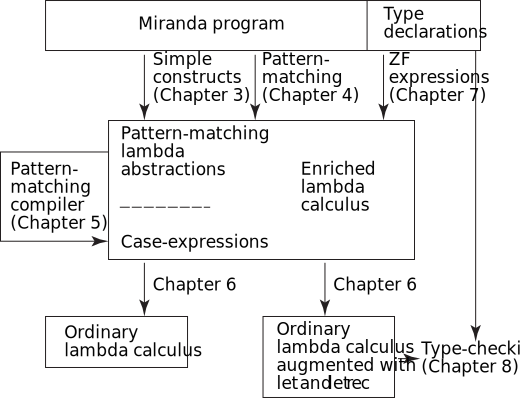
\includegraphics[width=0.96\textwidth]{chapters/Fig3_4}
%                    \includesvg{chapters/Fig3_4}
%                    \input{chapters/Fig3_4.tex}

            \end{minipage}%

    }%

    \caption{\textsf Organization of Chapters 4-8}
\end{figure}

\section*{References}

\begin{references}
    \item Gordon, M.J.C. 1979. \textit{The Denotational Description of Programming Languages}. Springer Verlag.
    \item Turner, D.A. 1985. Miranda -- a non-strict functional language with polymorphic types. In \textit{Conference on Functional Programming Languages and Computer Architecture, Nancy}, pp. 1-16, Jouannaud (editor). LNCS 201. Springer Verlag.
\end{references}

\chapter[Structured Types and the Semantics of Pattern-Matching][Structured Types and the Semantics of Pattern-Matching]{Structured Types and the\\Semantics of\\Pattern-Matching}
\chapterauthors{Simon L. Peyton Jones and Philip Wadler}
\vspace{3cm}


\noindent This chapter concerns structured types, a powerful and general mechanism
for defining data types, provided by several functional languages, including
Miranda, ML and Hope. Intimately associated with structured types is a
notational device known as pattern-matching, which is used by such
languages for defining functions.

Section 4.1 gives a general introduction to structured types and pattern-matching. Section 4.2 begins with a more in-depth look at pattern-matching
and conditional equations, and then introduces two new constructs in the
enriched lambda calculus, \fatbar{} and pattern-matching lambda abstractions. Using
these constructs, we then show how to translate a general Miranda function
definition into the enriched lambda calculus. Section 4.3 is devoted to
providing a precise semantics for pattern-matching lambda abstractions.

We conclude in Section 4.4 by defining case-expressions, the last new
construct of the enriched lambda calculus. This clears the way for Chapter 5,
which will show how to transform pattern-matching lambda abstractions into
case-expressions, thus giving a considerable gain in efficiency.

What in this chapter are called `structured types' are called `algebraic types'
in Miranda, and `free data types' by some others [Burstall and Goguen, 1982].

\section{Introduction to Structured Types}

Suppose that we wish to define binary trees with leaves that are numbers. In the notation of Miranda, this could be done by declaring a structured type tree as follows:
\begin{mlcoded}
    tree \typedecl{} \ml{LEAF} num | \ml{BRANCH} tree tree
\end{mlcoded}
(The symbol `\typedecl{}' identifies this as a type declaration.) This might be read as follows: `a tree is either a \ml{LEAF}, which contains a \ml{num}, or a \ml{BRANCH}, which contains a tree and a tree'. Here \ml{LEAF} and \ml{BRANCH} are called \textit{constructors} of the type. Miranda requires that constructors (and only constructors) begin with an upper-case letter, but we will always write them entirely in upper case. \ml{LEAF} has one \textit{field}, of type \ml{num}, and \ml{BRANCH} has two, both of type tree. The number of fields associated with a constructor is called its \textit{arity}; thus \ml{LEAF} has arity 1 and \ml{BRANCH} has arity 2.

Constructors can be used as functions, to create values of type \ml{tree}. For example, the following equation
\begin{mlcoded}
    tree1 $=$ BRANCH (BRANCH (LEAF 1) (LEAF 2)) (LEAF 3)
\end{mlcoded}
defines \ml{tree1} to be a \ml{tree}. Informally, this tree might be drawn as:
\begin{mlcoded}
\begin{center}
    \begin{forest}
        [. [. [1] [2]] [3]]
    \end{forest}
\end{center}
\end{mlcoded}

Constructors can also appear on the left-hand side of an equation, as in the following Miranda function definition:
\begin{mlcoded}
    \begin{tabular}{ll}
    reflect (LEAF n) &$=$ LEAF n \\
    reflect (BRANCH t1 t2) &$=$ BRANCH (reflect t2) (reflect t1)
    \end{tabular}
\end{mlcoded}
For example, \ml{(reflect tree1)} returns
\begin{mlcoded}
    BRANCH (LEAF 3) (BRANCH (LEAF 2) (LEAF 1))
\end{mlcoded}

A definition with patterns on the left-hand side, such as that of \ml{reflect}, is said to use \textit{pattern-matching} to perform \textit{case analysis}. For example, in evaluating \ml{(reflect t)} there are two cases to choose from: \ml{t} matches the pattern \ml{(LEAF n)}, or \ml{t} matches the pattern \ml{(BRANCH t1 t2)}. If, say, \ml{t} is \ml{(LEAF 1)} then the first case is chosen, with \ml{n} bound to \ml{1}. Much more will be said about pattern-matching later.

An important difference in the treatment of structured types in Miranda from that in ML or Hope, is that in Miranda constructor functions are lazy; that is, they do not evaluate their arguments. The components of a structured object are evaluated only when (and if) they are subsequently extracted and used, not when the object is built.

\subsection{Type Variables}

Type declarations may also contain type variables. For example, the definition of the type tree above may be rewritten to allow trees with leaves of any type:
\begin{mlcoded}
    tree $*$ \hastype$=$ \ml{LEAF} $*$ | \ml{BRANCH} (tree $*$) (tree $*$)
\end{mlcoded}
Here $*$ is called a \textit{generic} (or \textit{schematic}) \textit{type variable}. The declaration could be read as follows: `a tree of $*$ is either a \ml{LEAF}, which contains a $*$, or a \ml{BRANCH} which contains a tree of $*$ and a tree of $*$, for any type $*$'.

Leaves of any particular tree must all contain values of the same type, but different trees may have leaves of different types. Examples of trees and their types are
\begin{mlcoded}
    \begin{tabular}{ll}

    \ml{BRANCH} (\ml{LEAF} 1) (\ml{LEAF} 2)
    &\hastype tree num\\
    \ml{BRANCH} (\ml{LEAF} `a') (\ml{LEAF} `b')
    &\hastype tree char

    \end{tabular}
\end{mlcoded}
(The symbol \hastype is pronounced `has type'.) Here, `tree' is called a \textit{type-forming operator}, since it takes a type (such as \ml{num} or \ml{char}) as an `argument' and produces a type (respectively, \ml{(tree num)} or \ml{(tree char)}).

The repeated use of $*$ on the right-hand side of the type declaration specifies that the two branches of a tree must be of uniform type. For example,
\begin{mlcoded}
    \ml{BRANCH} (\ml{LEAF} 1) (\ml{LEAF} 'a')
\end{mlcoded}
is not legal, since it has leaves of mixed type. More will be said about types and type variables in Chapter 8.

\subsection{Special Cases}

This section shows how three `built-in' types, namely lists, tuples and enumerated types, can be regarded as instances of general structured types.

\subsubsection{Lists}

Miranda has a special syntax to denote lists, but lists are just an instance of a general structured type. Lists could be defined as follows:

\begin{mlcoded}
    list $*$ \hastype$=$ \ml{NIL} | \ml{CONS} $*$ (list $*$)
\end{mlcoded}

This type declaration defines the two new constructors \ml{NIL} and \ml{CONS}. Miranda's built-in syntax for lists could then be translated to use \ml{NIL} and \ml{CONS}, as follows:

\begin{quote}
    \ml{[ ]} is translated to \ml{NIL}\\
    \ml{(x:xs)} is translated to \ml{(CONS x xs)}.\\
    \ml{[x,y,z]} is a Miranda abbreviation for \ml{(x:y:z:[ ])} and hence is translated to
    \ml{(CONS x (CONS y (CONS z NIL)))}\\
    \ml{[$*$]} is translated to (list \ml{$*$})
\end{quote}

\begin{figure}[H]
\centering

{%
    \setlength{\fboxrule}{1pt}%
    \setlength{\fboxsep}{10pt}%
    \fbox{%
        \begin{minipage}{\textwidth}
            \footnotesize
\begin{mlcoded}
    \begin{tabular}{lll}
        \metafnbb{TE}{:}  &$\equiv$ &CONS \\
        \metafnbb{TE}{[ ]}  &$\equiv$ &NIL \\
        \metafnbb{TE}{[E$_1$, E$_2$, $\ldots$, E$_n$]}  &$\equiv$ &CONS \metafnbb{TE}{E$_1$} \metafnbb{TE}{[E$_2$, $\ldots$, E$_n$]}\\
        \metafnbb{TE}{(E$_1$, E$_2$)}  &$\equiv$ &PAIR \metafnbb{TE}{E$_1$} \metafnbb{TE}{E$_2$} \\
        \metafnbb{TE}{(E$_1$, E$_2$, E$_3$)}  &$\equiv$ &TRIPLE \metafnbb{TE}{E$_1$} \metafnbb{TE}{E$_2$} \metafnbb{TE}{E$_3$}\\
        {\normalfont\normalsize and so on} & & \\
        \metafnbb{TE}{True}  &$\equiv$ &TRUE \\
        \metafnbb{TE}{False}  &$\equiv$ &FALSE \\
    \end{tabular}
\end{mlcoded}
        \end{minipage}%
    }%
}%

\caption{\textsf Modifications to the TE scheme for lists, tuples and booleans}
\end{figure}

\noindent(Note: the last example is different from the others, because it describes a type-expression rather than a value-expression.)

We can conveniently perform this translation when translating from Miranda into the enriched lambda calculus; Figure 4.1 gives the required equations.

Notice that the elements of a list of type \ml{(list $*$)} must all be of type \ml{$*$}, but the number of elements in a list is not determined by its type. Thus \ml{(CONS} 2 \ml{NIL)} and \ml{(CONS 3 (CONS 6 NIL)} are both of type \ml{(list num)}, though they are of different lengths.

\subsubsection{Tuples}

Miranda also provides special syntax to denote tuples, and these also can be defined using a structured type. Tuples could be defined as follows:

\begin{mlcoded}
    \footnotesize
    \begin{tabular}{llll}
    pair        & $*\ **$           &\typedecl{} PAIR        & $*\ **$ \\
    triple      & $*\ **\ ***$       &\typedecl{} TRIPLE      & $*\ **\ ***$ \\
    quadruple   & $*\ **\ ***\ ***$   &\typedecl{} QUADRUPLE   & $*\ **\ ***\ ***$
    \end{tabular}
\end{mlcoded}

Notice the difference between `\ml{pair}' and \ml{PAIR}: the former is a type-forming operator, used only in type-expressions, while the latter is the constructor function of the type, used only in value-expressions.

As with lists, Miranda's special syntax can be translated as follows:
\begin{quote}
    \ml{(x,y)} is translated to \ml{(PAIR x y)}\\
    \ml{(x,y,z)} is translated to \ml{(TRIPLE x y z)}\\
    and so on.\\
    \ml{($*$, $**$)} is translated to (pair $*$ $*$ $*$)\\
    \ml{($*$, $**$, $***$)} is translated to \ml{(triple $*$ $**$ $***$)}
\end{quote}
Figure 4.1 gives the required equations.

Notice that a tuple may contain elements of mixed type; for example
\begin{mlcoded}
\begin{tabular}{ll}
    (3, TRUE) &\hastype{} PAIR num bool\\
    (`a', (3, 2)) &\hastype{} PAIR char (PAIR num num)
\end{tabular}
\end{mlcoded}
However, the type of a tuple completely determines the number and the types
of its fields. For example, a \ml{pair} always contains exactly two fields, a \ml{triple}
contains exactly three fields, and so on.

\subsubsection{Enumerated types}

The type declaration

\begin{mlcoded}
    color \hastype$=$ \ml{VERMILLION} | \ml{PUCE} | \ml{LAVENDER}
\end{mlcoded}
in which each constructor has zero fields, is just like an enumerated type in Pascal. Thus, we can define the type of boolean values:
\begin{mlcoded}
    bool \hastype$=$ \ml{TRUE} | \ml{FALSE}
\end{mlcoded}

The usual functions on booleans can then be defined using pattern-matching; for example:
\begin{mlcoded}
    \begin{tabular}{ll}
    if \ml{TRUE} &e1 e2 $=$ e1\\
    if \ml{FALSE} &e1 e2 $=$ e2
    \end{tabular}
\end{mlcoded}

Miranda uses the names `\ml{True}' and `\ml{False}' for its built-in truth-values.

\subsubsection{Summary}

Since it is easy to translate `built-in' types like lists and tuples into equivalent structured types, then any implementation of a functional language that handles structured types will also handle these `built-in' types for free. This can greatly simplify an implementation. Instead of implementing several type mechanisms, one for lists, one for tuples, one for enumerated types, and so on, we need only implement a single mechanism for structured types, and translate other types into structured types. Figure 4.1 gives the required equations.

\subsection{General Structured Types}

In general, the form of a structured type definition is:

\begin{mlcoded}
    T \hastype$=$ c$_1$ T$_{1,1}$ $\ldots$ T$_{1,r_1}$\\
    \quad | $\ldots$\\
    \quad | c$_n$ T$_{n,1}$ $\ldots$ T$_{n,r_n}$\\
\end{mlcoded}
where the \ml{T$_{i,j}$} are types and the \ml{c$_i$} are constructors of arity $r_i$. In the `\ml{tree}' example above, \ml{T} was \ml{(tree $*$)}, \ml{c$_1$} was \ml{LEAF}, \ml{T$_{1,1}$} was \ml{num}, \ml{c$_2$} was \ml{BRANCH}, \ml{T$_{2,1}$} was \ml{(tree $*$)}, and \ml{T$_{2,2}$} was \ml{(tree $*$)}.

Readers familiar with the mathematical operations for constructing types will recognize that the general type above can be written as the sum (that is, discriminated union):
\begin{mlcoded}
T $=$ T$_1$ $+ \ldots +$ T$_n$
\end{mlcoded}
where each \ml{T$_i$}, for $i$ from 1 to $n$, can be written as a product:
\begin{mlcoded}
T$_i =$ T$_{i,1} \times$ T$_{i,2} \times \cdots \times$ T$_{i,r_i}$
\end{mlcoded}
In other words, a structured type is a \textit{sum-of-products}.

When $n=1$ we say that the type is a \textit{product type}; the types \ml{(pair $*\ **$)}, \ml{(triple $*\ **\ ***$)}$\ldots$ are all product types. When $n>1$ we say that the type is a \textit{sum type}, since it is the sum of more than one domain; the types \ml{(tree $*$)}, \ml{(list $*$)}, \ml{color} and \ml{bool} are all sum types. Thus a product type has exactly one constructor, and a sum type has two or more constructors.

We will often wish to distinguish between the constructors of product types and sum types. Just as we use the names \ml{c$_i$} to stand for constructors of all types, we will use the name \ml{t} to stand for the constructor of a product type, and the names \ml{s} and \ml{s$_i$} to stand for the constructors of a sum type (\ml{t} suggests `tuple' and \ml{s} suggests `sum').

(Note: we use lower-case letters to stand for constructors, to avoid confusion with the constructors themselves, which are written in upper case. Similarly, we use upper-case letters to stand for types, which are themselves written in lower case $-$ see Section 4.1.)

(\textit{Important:} at the time when this chapter was first written the semantics of Miranda provisionally specified that a structured type with only one constructor was a product type, as above. However, an alternative view is that a structured type with only one constructor should behave as a sum type with one component in the sum, and that product types (tuples) be treated as an independent construct. It now seems likely that Research Software Limited will follow this latter course in their definition of Miranda. As a consequence some of the statements made in this chapter about the semantics of structured types in Miranda may be incorrect. We draw the reader's attention to the caveat on page 37.)

\subsection{History}

As mentioned, structured types are a combination of sum types and product types, which have a long history in mathematics.

Landin's Iswim, one of the earliest functional languages, was described using a stylized form of English for defining structured types [Landin, 1966]. Burstall introduced a more formal notation for defining such types in NPL [Burstall, 1977]. Hope and ML have type systems based on separate sum and product types, whereas Miranda and Orwell have type systems based on sum-of-product types.

Iswim also contained a simple form of pattern-matching, where one could write definitions such as
\begin{mlcoded}
    addPair (x,y) $=$ x $+$ y
\end{mlcoded}
However, the important idea of using pattern-matching for case analysis appears to have been developed independently by Burstall and Turner. Pattern-matching appeared in NPL and SASL, and was used to good effect in proofs by structural induction [Burstall, 1969] and program transformation
[Burstall and Darlington, 1977]. It was incorporated into many later
languages such as Hope, KRC, ML, Miranda and Orwell.

\section{Translating Miranda into the Enriched Lambda Calculus}

We must now demonstrate how to translate Miranda function definitions involving pattern-matching into the enriched lambda calculus. In the process of doing so we will introduce \textit{pattern-matching lambda abstractions} and the \fatbar operator, two of the constructs in the enriched lambda calculus whose explanation was postponed.

\subsection{Introduction to Pattern-matching}
We begin this section by illustrating some further aspects of pattern-matching, which have to be handled by an implementation. (Not all the illustrations should be taken as examples of good programming style. Some are expressly chosen to demonstrate all the possible nasty things that can happen!)  Recall the definition of \ml{reflect}:
\begin{mlcoded}
    \begin{tabular}{ll}
    reflect (LEAF n) &$=$ LEAF n\\
    reflect (BRANCH t1 12) &$=$ BRANCH (reflect 12) (reflect t1)
    \end{tabular}
\end{mlcoded}

The terms \ml{(LEAF n)} and \ml{(BRANCH t1 12)} occurring on the left-hand side of these equations are called \textit{patterns}. When \ml{reflect} is applied to an argument, the argument is first evaluated to see whether it \textit{matches} the pattern \ml{(LEAF n)} or \ml{(BRANCH t1 12)}. It will certainly match one or the other, because the type-checker ensures that \ml{reflect} is only applied to objects of type \ml{(tree $*$)}, for some type \ml{$*$}. For example, if \ml{reflect} is applied to an expression which evaluates to \ml{(BRANCH E$_1$ E$_2$)}, the second equation is selected, with \ml{t1} bound to \ml{E$_1$} and \ml{12} bound to \ml{E$_2$}.

In the preceding example, the order in which the equations were written was immaterial, but this is not always the case. Consider the Miranda function definition
\begin{mlcoded}
    factorial 0 $=$ 1\\
    factorial n $=$ n $*$ factorial (n-1)
\end{mlcoded}

The order of the equations in this definition is significant. In the evaluation of \ml{(factorial x)}, there are two cases to choose from: either \ml{x} matches \ml{0} (that is, \ml{x} evaluates to \ml{0}), so the first equation is chosen, or it does not, so the second case is chosen with \ml{n} bound to \ml{x}. The equations are tried out one at a time, from top to bottom. If they had been written in the other order then the first equation would always match. In this situation we say that the patterns \textit{overlap}. (As we shall see in Chapter 5, there are good reasons to avoid writing overlapping patterns, but occasionally they prove useful.)

Another point, illustrated by the first \ml{factorial} equation, is that a pattern may consist of a literal constant, such as a number or character.

As another example, consider the Miranda function definition
\begin{mlcoded}
    \begin{tabular}{ll}
    lastElt (x:[]) &$=$ x\\
    lastElt (x:xs) &$=$ lastElt xs
    \end{tabular}
\end{mlcoded}
The function call \ml{(lastElt xs)} returns the last element of the list \ml{xs}. Again, the order of the equations is significant, since the patterns overlap. Furthermore, the first pattern is an example of a \textit{nested} pattern, in which the pattern \ml{[\,]} is nested inside the pattern \ml{(x:[\,])}. Finally, the equations are not exhaustive, since neither pattern matches the argument \ml{[\,]}. If \ml{lastElt} is applied to \ml{[\,]} some sort of error should be reported.

Pattern-matching can apply to several arguments, as the following Miranda definition shows:
\begin{mlcoded}
    \begin{tabular}{lll}
    xor False &y &$=$ y\\
    xor True &False &$=$ True\\
    xor True &True &$=$ False
    \end{tabular}
\end{mlcoded}

Another feature of Miranda that is closely connected with pattern-matching is \textit{conditional equations}, which control the selection of \textit{alternatives} by the use of \textit{guards}. We could, for example, rewrite the \ml{factorial} function in the following way:
\begin{mlalign}
    factorial n & $=$ 1,\qquad n=0\\
              n & $=$ n $*$ factorial (n-1)
\end{mlalign}
A single left-hand side governs several alternatives, which together constitute the right-hand side. In this case there is only one guard, namely the boolean-valued expression `\ml{n=0}', which appears following a comma. Guards are evaluated one at a time, beginning at the top, and when a guard evaluates to \ml{True}, the corresponding alternative expression is selected. The guard may be omitted in the final right-hand side, giving an `otherwise' case (equivalent to a guard of \ml{True}).

The \ml{factorial} example shows, incidentally, that a constant appearing in a pattern can easily be eliminated by replacing it with a variable and adding a guard to the equation instead.

Conditional equations interact with pattern-matching, as demonstrated in the next example. The function \ml{funnyLastElt} returns the last element of its argument list, except that if a negative element is encountered then it is returned instead:
\begin{mlcoded}
    \begin{tabular}{ll}
        funnyLastElt (x:xs) &$=$ x,\qquad x<0\\
        funnyLastElt (x:[]) &$=$ x\\
        funnyLastElt (x:xs) &$=$ funnyLastElt xs
    \end{tabular}
\end{mlcoded}
Pattern-matching proceeds, as usual, from top to bottom; when a left-hand side matches the argument, the guarded alternative(s) are tried, from top to bottom. If none of the guards is \ml{True}, then pattern-matching continues, Starting with the next equation. Applying \ml{funnyLastElt} to the list \ml{[1,2]} would cause this behavior, since the first equation would match, but the guard fails, so the second and then third equations are tried.

Finally, variables may be repeated on the left-hand side of an equation. For example, the function \ml{noDups} eliminates adjacent duplicate elements in a list:
\begin{mlcoded}
    \begin{tabular}{ll}
    noDups [\,] &$=$ [\,]\\
    noDups [x] &$=$ [x]\\
    noDups (x:x:xs) &$=$ noDups (x:xs)\\
    noDups (x:y:ys) &$=$ x : noDups (y:ys)
    \end{tabular}
\end{mlcoded}
The third equation matches only if the first two elements of the argument list are equal; the repeated use of \ml{x} on the left-hand side implies the equality condition.

We may summarize the features that the implementation must support as follows:
\begin{numbered}
    \item overlapping patterns;
    \item constant patterns;
    \item nested patterns;
    \item multiple arguments;
    \item non-exhaustive sets of equations;
    \item conditional equations;
    \item repeated variables.
\end{numbered}
Given these complications, it is unwise to rely on a purely intuitive understanding of what a function definition using pattern-matching means. The rest of this section and the next is therefore devoted to providing a formal semantics of pattern-matching.

\subsection{Patterns}
First of all, we will need a precise definition of patterns.

\definitionbox{{\normalfont A pattern \ml{p} is}}{
\begin{tabular}{ll}
    either & a variable \ml{v}\\
    or     & a constant \ml{k}, such as a number, a character, a boolean and so on,\\
    or &a constructor pattern, of the form \ml{(c p$_1$ \ldots p$_r$)} where \ml{c} is a\\
    & constructor of arity \ml{r}, and p$_1,\, \ldots,\, $p$_r$ are themselves patterns.
\end{tabular}
\vspace{0.25\baselineskip}

All of the variables in a pattern should be distinct.

A pattern of the form \ml{(s p$_1$ \ldots p$_r$)}, where \ml{s} is a sum constructor, is called a \textit{sum-constructor pattern}, or \textit{sum pattern}. A pattern of the form \ml{(t p$_1$ \ldots p$_r$)}, where \ml{t} is a product constructor, is called a \textit{product-constructor pattern}, or \textit{product pattern}.
\vspace{0.25\baselineskip}

\noindent Note: according to this definition, patterns may not contain repeated variables, although Miranda allows them to do so. This point is discussed in Section 4.2.7.
}

Here are some examples of patterns:

\begin{tabular}{ll}
\ml{x} & \\
\ml{LEAF n} & \\
\ml{BRANCH (LEAF n) t} & \\
\ml{CONS x xs} & (written \ml{(x:xs)} in Miranda) \\
\ml{CONS x (CONS 3 NIL)} & (written \ml{[x,3]} in Miranda) \\
\ml{PAIR x 4} &(written \ml{(x,4)} in Miranda)
\end{tabular}

\noindent The term \ml{(PAIR z z)} is not a pattern, because it contains a repeated variable. The term \ml{(CONS x)} is not a pattern, because the \ml{CONS} does not have enough arguments.

Miranda allows patterns with repeated variables, like \ml{(PAIR z z)} but the patterns defined here do not. This is discussed in Section 4.2.7.

A constructor pattern is \textit{simple} if it has the form \ml{(c v$_1$ $\ldots$ v$_r$)}, where \ml{v$_1$, $\ldots$, v$_r$} are distinct variables. If a constructor pattern is not simple it is \textit{nested}.

\subsection{Introducing Pattern-matching Lambda Abstractions}

Up to now we have translated function definitions into the lambda calculus using the following rule:
\begin{mlcoded}
	\metafnbb{TD}{f v$_1$ ... v$_n$ $=$ E}   $\equiv$ f $=$ \tl{}v1\ldots\tlb{v$_n$}\metafnbb{TE}{E}
\end{mlcoded}
where \ml{v$_1$, $\ldots$, v$_n$} are variables. Temporarily restricting our attention to functions of a single variable, we could derive the less general rule
\begin{mlcoded}
	\metafnbb{TD}{f v $=$ E} $\equiv$ f $=$ \tlb{v}\metafnbb{TE}{E}
\end{mlcoded}
By analogy, given the function definition
\begin{mlcoded}
	\ml{f p $=$ E}
\end{mlcoded}
(where \ml{p} is a pattern), it seems plausible to translate it using the rule
\begin{mlcoded}
	\metafnbb{TD}{f p $=$ E} $\equiv$ f $=$ \tlb{p}\metafnbb{TE}{E}
\end{mlcoded}

This is not quite right yet, because we must remember to translate the pattern, so that Miranda's list notation is translated into uses of \ml{CONS} and \ml{NIL} (and likewise for tuples and booleans). Fortunately, the syntax of patterns is a subset of that of expressions, so we can use the \metafn{TE} scheme.
\begin{mlcoded}
	\metafnbb{TD}{f p $=$ E} $\equiv$ f $=$ \tlb{\metafnbb{TE}{p}}\metafnbb{TE}{E}
\end{mlcoded}
For example, consider the Miranda function definition for \ml{fst}:
\begin{mlcoded}
	fst (x, y) $=$ x
\end{mlcoded}
Using the rule above gives:
\begin{mlcoded}
	\metafnbb{TD}{fst (x, y) $=$ x} $\equiv$ fst $=$ \tlb{(PAIR x y)}x
\end{mlcoded}
This introduces a new sort of lambda abstraction, a \textit{pattern-matching lambda abstraction}, which has the form \ml{(\tlb{p}E)} where \ml{p} is a pattern. This leaves us with two questions:
\begin{numbered}
	\item How can we translate a general Miranda function definition into pattern-matching lambda abstractions?
	\item What, exactly, does \ml{(\tlb{p}E)} mean?
\end{numbered}
We discuss the first in the remainder of this section, leaving the second for the next section.

\subsection{Multiple Equations and Failure}

Consider first a Miranda function definition of the form
\begin{mlcoded}
	f p$_1$ $=$ E$_1$\\
	f p$_2$ $=$ E$_2$\\
	$\cdots$\\
	f p$_n$ $=$ E$_n$
\end{mlcoded}
Intuitively, we expect the semantics to be `try the first equation, and if that fails try the second, and so on'. This introduces the idea that a pattern-match might \textit{fail}. Such failure does not necessarily indicate an error, since there might be a subsequent equation which would match. Hence, we introduce a new built-in value \ml{FAIL}, which is returned when a pattern-match fails.

With the aid of this idea, we can translate the definition of \ml{f} into the following enriched lambda calculus expression:

\begin{mlalign}
	f $=$  \tlb{x}&(  (( \tlb{p$_1'$}E$_1'$) x)\\
	& \fatbar{} (( \tlb{p$_2'$}E$_2'$)  x)\\
	& $\cdots$ \\
	& \fatbar{} (( \tlb{p$_n'$}E$_n'$)  x)\\
	& \fatbar{} ERROR )
\end{mlalign}

where \ml{x} is a new variable name that does not occur free in any \ml{E$_i$}, the expressions \ml{E$_i'$} are the result of translating the \ml{E$_i$}, and the patterns \ml{p$_i'$} are the result of translating the \ml{p$_i'$}. The new definition of \ml{f} can be read `try to apply \ml{(\tlb{p$_1'$}E$_1'$)} to \ml{x}, and if that succeeds return its result; otherwise try \ml{(\tlb{p$_2'$}E$_2'$)}, and so on; if they all fail, return \ml{ERROR}'.

Here \ml{ERROR} is meant to be a special value whose evaluation indicates an error, an event which should never occur.

The function \ml{\fatbar{}} is an infix function, whose behavior is described by the semantic equations:
\begin{mlcoded}
	\begin{tabular}{ll}
		a &\fatbar{} b $=$ a \qquad {\normalfont if} a $\neq \bot$ {\normalfont and} a $\neq$ FAIL\\
	FAIL & \fatbar{} b $=$ b  \\
	$\bot$ & \fatbar{} b $= \bot$
	\end{tabular}
\end{mlcoded}

Operationally, \fatbar{} evaluates its left argument; if the evaluation terminates and yields something other than \ml{FAIL}, then \fatbar{} returns that value (first rule); if it evaluates to \ml{FAIL}, \fatbar{} returns its right argument (second rule); if the evaluation of the left argument fails to terminate, then so does the application of \fatbar{} (third rule).

It is easy to verify that \fatbar{} is an \textit{associative} operator, and has \textit{identity} \ml{FAIL}. Its associativity means that we may write expressions such as \ml{(E$_1$ \fatbar{} E$_2$ \fatbar{} E$_3$)} without ambiguity. It is extremely convenient to write \fatbar{} between its operands (that is, infix) but, since all functions are written prefix in the lambda calculus, we are forced to dignify \fatbar{} by making it one of the new constructs of the enriched lambda calculus. The sole reason for doing so is notational.

As an example of the suggested translation in action, recall the definition of the \ml{reflect} function:
\begin{mlcoded} \footnotesize
    \begin{tabular}{ll}
    reflect (LEAF n) &$=$ LEAF n \\
    reflect (BRANCH t1 t2) &$=$ BRANCH (reflect t2) (reflect t1)
    \end{tabular}
\end{mlcoded}
This would be translated to:
\begin{mlalign}\footnotesize
    \tlb{reflect} $=$ &\tlb{t}( ((\tlb{(LEAF n)}LEAF n) t) \\
    &\fatbar{} ((\tlb{(BRANCH t1 t2)}BRANCH (reflect t2) (reflect t1)) t)\\
    &\fatbar{} ERROR )
\end{mlalign}

In this case, of course, \ml{ERROR} can never be returned, since one of the previous pattern-matches will succeed. This is not always the case, as the following example shows. Consider the Miranda definition of \ml{hd}, which extracts the first element of a list:
\begin{mlcoded}
    hd (x:xs) $=$ x
\end{mlcoded}
It would be translated to
\begin{mlcoded}
    hd $=$ \tlb{xs'}(((\tlb{(CONS x xs)}x) xs') \fatbar{} \ml{ERROR})
\end{mlcoded}
If \ml{hd} is applied to \ml{NIL}, then \ml{ERROR} will be the result. (We have used \ml{xs'} as the formal parameter of the lambda abstraction, to avoid confusion with the \ml{xs} in the pattern. Technically, however, there would be no problem with using \ml{xs}, or any other variable, since \ml{hd} has no free variables.)

\subsection{Multiple Arguments}

Functions with multiple arguments are easily handled. As we recalled earlier, the basic approach is to translate a function of several arguments using the rule
\begin{mlcoded}
    \metafnbb{TD}{f v$_1$ $\ldots$ v$_n$ $=$ E} $\equiv$ f $=$ \tlb{v$_1$}$\cdots$\tlb{v$_n$}\metafnbb{TE}{E}
\end{mlcoded}
Combining this with the approach of the previous section suggests that we should translate the definition
\begin{mlcoded}
    \ml{f p$_1$ p$_2$ $\ldots$ p$_m$ $=$ E}
\end{mlcoded}
where \ml{p$_1$, $\ldots$, p$_m$} are patterns, into
\begin{mlcoded}
    f $=$ \tl{}v$_1\ldots$ \tlb{v$_m$}(((\tl{}p$_{1}'\ldots$\tlb{p$_{m}'$}E$'$) v$_1 \ldots$ v$_m$) \fatbar{} ERROR)
\end{mlcoded}
where \ml{v$_1$, $\ldots$, v$_m$} are new variables that do not occur free in \ml{E}, the \ml{p$_{i}'$} are the results of translating the \ml{p$_i$}, and \ml{E$'$} is the result of translating \ml{E}. The only new complication is that we must specify what happens in case of failure. Suppose \ml{f} is applied to \ml{m} arguments, and the first pattern-match fails:
\begin{mlcoded}
    (\tl{}p$_{1}' \ldots$\tlb{p$_{m}'$}E$'$) E$_1$ E$_2 \ldots$ E$_m \rightarrow$ FAIL E$_2 \ldots$ E$_m$
\end{mlcoded}

Then we want the whole expression to fail, so we need to add a reduction rule for \ml{FAIL}:
\begin{mlcoded}
    FAIL E $\rightarrow$ FAIL
\end{mlcoded}
Now we can continue reduction.
\begin{mlcoded}
    \ml{FAIL} E$_2$ E$_3\ldots$ E$_m$ $\rightarrow$ \ml{FAIL} E$_3\ldots$ E$_m$ $\rightarrow \cdots \rightarrow$ FAIL
\end{mlcoded}
The translation is readily extended for the case when \ml{f} is defined by several equations. To see an example of this in action, consider the definition of \ml{xor} given above:
\begin{mlcoded}
    \begin{tabular}{lll}
    xor False &y &$=$ y\\
    xor True &False &$=$ True\\
    xor True &True &$=$ False
    \end{tabular}
\end{mlcoded}
Combining the rules of this section and the last allows us to transform this to
\rightline{\footnotesize(Notice that the arguments are matched from left to right)}
\vspace{-\baselineskip}
\begin{mlalign}
    xor $=$ \tlb{x}\tlb{y}&( ((\tlb{FALSE}\tlb{y}y) x y) \\
    & \fatbar{} ((\tlb{TRUE}\tlb{FALSE}TRUE) x y) \\
    & \fatbar{} ((\tlb{TRUE}\tlb{TRUE}FALSE) x y) \\
    & \fatbar{} ERROR)
\end{mlalign}


\subsection{Conditional Equations}

Next, we describe how to translate conditional equations into the enriched lambda calculus. Consider the following Miranda definition:
\begin{mlcoded}
    \begin{tabular}{lll}
        gcd a b &$=$ gcd (a $-$ b) b, &a $>$ b\\
        &$=$ gcd a (b $-$ a), &a $<$ b\\
        &$=$ a, &a $=$ b
    \end{tabular}
\end{mlcoded}
It is easy to see that the right-hand side of this definition could be translated to
\begin{mlcoded}
    (IF ($>$ a b) (gcd ($-$ a b) b)\\
    (IF ($<$ a b) (gcd a ($-$ b a))\\
    (IF ($=$ a b) a FAIL)))
\end{mlcoded}
Notice that if all the guards fail, then \ml{FAIL} is returned by the nested \ml{IF} expression. (In the case of \ml{gcd} this can never occur, and a very clever compiler might be able to discover this fact and optimize the last \ml{IF}.) In a more complicated definition, the failure of all the guards would cause the next equation to be tried (see example below).

Regarding all of an equation after the first \ml{$=$} sign as a `right-hand side', we can now give a new translation scheme, \metafn{TR}, which translates right-hand sides:

\plainbox{
    {\centering

    \metafnbb{TR}{rhs} translates the right-hand side of a definition

    }

    \metafn{TR}\ml{\hspace{-2em}
        \begin{minipage}{0.3\textwidth}
        \[
            \left[\hspace{-4pt}\left[
            \begin{array}{rl}
                & \text{A}_1, \text{G}_1\\
                =& \text{A}_2, \text{G}_2\\
                & \cdots \\
                =& \text{A}_n, \text{G}_n
            \end{array}
            \right]\hspace{-4pt}\right]
            \equiv
        \]
        \end{minipage}
    }
    \begin{minipage}{0.6\textwidth}
        \vs
      \begin{mlcoded}
          (IF \metafnbb{TE}{G$_1$} \metafnbb{TE}{a$_1$} \\
          (IF \metafnbb{TE}{G$_2$} \metafnbb{TE}{a$_2$} \\
          (IF \metafnbb{TE}{G$_n$} \metafnbb{TE}{a$_n$} FAIL)$\cdots$ ))
      \end{mlcoded}
    \end{minipage}\vs

    where \ml{A$_i$} is an expression and \ml{G$_i$} is a boolean-valued expression.
}


Now we can use \metafn{TR} instead of \metafn{TE} to translate the right-hand sides of function definitions. As an example, recall the definition of \ml{funnyLastElt}:
\begin{mlcoded}
    \begin{tabular}{ll}
    funnyLastElt (x:xs) &$=$ x, x < 0\\
    funnyLastElt (x:[]) &$=$ x\\
    funnyLastElt (x:xs) &$=$ funnyLastElt xs
    \end{tabular}
\end{mlcoded}
We can now translate it to
\begin{mlalign}
    funnyLastElt $=$ \tlb{v}&( ((\tlb{CONS x xs} . IF (< x 0) x FAIL) v) \\
    &\fatbar{} ((\tlb{CONS x NIL}x) v)  \\
    &\fatbar{} ((\tlb{CONS x xs}funnyLastElt xs) v)  \\
    &\fatbar{} ERROR)
\end{mlalign}
If the first equation matches, but the guard fails, then the \ml{IF} returns \ml{FAIL}, and the next equation is tried.

In Miranda, the final guard \ml{G$_n$} may be omitted, which is equivalent to giving a final guard of \ml{True}. In this case, the innermost \ml{IF} is of the form
\begin{mlcoded}
    IF TRUE E$_1$ FAIL
\end{mlcoded}
which can be optimized to
\begin{mlcoded}
    E$_1$
\end{mlcoded}
For example, the definition of \ml{factorial}
\begin{mlalign}
    factorial n &$=$ 1, \qquad n $=$ 0\\
    &$=$ n $*$ factorial (n-1)
\end{mlalign}
would be translated to
\begin{mlalign}
    factorial $=$ \tlb{v}&( ((\tlb{n}IF ($=$ n 0) 1 ($*$ n (factorial ($-$ n 1)))) v)\\
     &\fatbar{} ERROR)
\end{mlalign}
This can be simplified further, since the pattern-match cannot fail, and this special case will be spotted by the transformations of Chapter 5.

\subsection{Repeated Variables}

It appears at first that it is easy to use a conditional equation to eliminate repeated variables, by introducing a new variable name to replace one of the occurrences of the repeated variable, and adding an appropriate equality condition. For example, we could rewrite the definition of \ml{noDups} (given in Section 4.2.1) thus:

\begin{mlcoded}
\begin{tabular}{ll}
    noDups [\,] &$=$ [\,]\\
    noDups [x] &$=$ [x]\\
    noDups (x:y:ys) &$=$ noDups (y:ys), x $=$ y\\
    noDups (x:y:ys) &$=$ x : noDups (y:ys)
\end{tabular}
\end{mlcoded}

(The last two equations could now be combined into a conditional equation with two alternatives.) Unfortunately, this approach occasionally conflicts with the left-to-right rule originally given for pattern-matching. For example, given the following definition:

\begin{mlcoded}
\begin{tabular}{ll}
    nasty x x True &$=$ 1\\
    nasty x y z &$=$ 2
\end{tabular}
\end{mlcoded}
consider the evaluation of
\begin{mlcoded}
    nasty bottom 3 False
\end{mlcoded}
where the evaluation of \ml{bottom} fails to terminate (for example, \ml{bottom} could be defined by the degenerate equation: \ml{bottom $=$ bottom}). We might expect that the evaluation \ml{(nasty bottom 3 False)} would not terminate, since we will try to evaluate \ml{bottom} in order to compare it with \ml{3}. However, suppose we transformed the definition of \ml{nasty} to use a conditional equation:
\begin{mlcoded}
\begin{tabular}{ll}
    nasty$'$ x y True &$=$ 1,\qquad x $=$ y\\
    nasty$'$ x y z &$=$ 2
\end{tabular}
\end{mlcoded}
Now, if we evaluate \ml{(nasty$'$ bottom 3 False)}, \ml{bottom} will match \ml{x} and \ml{3} will match \ml{y}, but the match of \ml{True} against \ml{False} will fail, so the second equation will be tried, and deliver the answer 2. Hence, \ml{nasty} and \ml{nasty$'$} behave differently, and the transformation is invalid. (Note: \ml{nasty} and \ml{nasty$'$} also behave differently for expressions such as \ml{(nasty 1 2 bottom)}.)

There is a further complication raised by repeated variables. Consider the function \ml{multi}:
\begin{mlcoded}
\begin{tabular}{ll}
        multi p q q p $=$ 1\\
    multi p q r s $=$ 2
\end{tabular}
\end{mlcoded}

Should we compare the first and fourth arguments, and then compare the second and third arguments, or the other way around? The order of comparison is important, because it affects termination; consider \ml{(multi bottom 2 3 4)}.

This section has shown that repeated variables in a pattern are not as straightforward as at first appeared (the examples were suggested by Simon Finn of the University of Stirling). To simplify the rest of this chapter we will therefore sidestep these complications, by restricting our attention to a subset of Miranda which does not allow repeated variables in a pattern. We lose no expressive power thereby, though we do lose some notational convenience.

\subsection{Where-clauses}
Miranda allows the right-hand side of a definition to be qualified with a \ml{where}-clause. For example,
\begin{mlalign}
    sumsq x y $=$ xsq $+$ ysq&\\
    where\qquad{} &\\
    xsq &$=$ x $*$ x\\
    ysq &$=$ y $*$ y
\end{mlalign}
It is intuitively clear that this could be translated to
\begin{mlalign}
    sumsq $=$ \tlb{x}\tlb{y}(let &xsq $=$ $*$ x x\\
    &ysq $=$ $*$ y y\\
    in &\\
    & ($+$ xsq ysq))
\end{mlalign}
where we use a \ml{let}-expresion instead of a \ml{where}-clause. In general, the definitions in a \ml{where}-clause may be mutually recursive, so we have to use a \ml{letrec}-expresion instead. This will be optimized in Section 6.2.8.

Finally, the scope of a where-clause may include a set of alternatives and guards in a conditional equation:
\begin{mlcoded}
    \begin{tabular}{rll}
        gcd a b $=$ &gcd diff b, &a $>$ b\\
        $=$ &gcd a ($-$diff), &a $<$ b\\
        $=$ &a, & a $=$ b\\
        &where & \\
        & \qquad diff $=$ a $-$ b &
    \end{tabular}
\end{mlcoded}

% Figure 4.2 has been relocated to be with 4.3 and 4.4.

The scope of the definition of \ml{diff} includes all the alternatives and guards.
Figure 4.2 gives the final \metafn{TR} translation scheme, which translates right-hand sides, using a \ml{letrec} to translate a \ml{where}-clause.

\subsection{Patterns on the Left-hand Side of Definitions}

So far we have only described how to translate \textit{function} definitions, but Miranda also allows a \textit{pattern} to appear on the left-hand side of a definition. For example, consider the following Miranda definition:
\begin{mlalign}
    addPair w $=$ x $+$ y & \\
    where &(x, y) $=$ w
\end{mlalign}
The product pattern \ml{(x, y)} appears on the left-hand side of the definition in the \ml{where}-clause. It implies that \ml{w} evaluates to a pair, and it binds the names \ml{x} and \ml{y} to the components of \ml{w}.

As mentioned in Section 3.2.3, we also allow general patterns to appear on the left-hand side of definitions in a \ml{let(rec)}. This extension allows us to make a simple translation of \ml{addPair} to
\begin{mlcoded}
    addPair $=$ \tlb{w}(letrec (PAIR x y) $=$ w in ($+$ x y))
\end{mlcoded}

The hard work of dealing with patterns on the left-hand side of definitions is now carried out by transforming this \ml{letrec} into the ordinary lambda calculus, which is described in Section 6.2. The modification required to \metafn{TD} is very simple:
\begin{mlcoded}
    \metafnbb{TD}{ p $=$ R } $\equiv$ \metafnbb{TE}{p} $=$ \metafnbb{TR}{R}
\end{mlcoded}
where \ml{p} is a pattern and \ml{R} is a right-hand side.

\subsection{Summary}
We have now completed the development of the translation of a significant subset of Miranda into the enriched lambda calculus. The final translation schemes, summarized in Figures 4.2, 4.3 and 4.4, look rather forbidding, but this is because of their generality rather than their complexity.

\section{The Semantics of Pattern-matching Lambda Abstractions}
Having described how to translate from Miranda into a language involving pattern-matching lambda abstractions, we now give the semantics of pattern-matching lambda abstractions of the form \ml{( \tlb{p}E)}.

We will do so by devoting a subsection to each form of the pattern, \ml{p}: variable, constant, sum-constructor, and product-constructor.


\boxedfigure{
    {\centering

        \metafnbb{TR}{rhs} translates the right-hand side of a definition

    }

    \hspace{-1em}\metafn{TR}\ml{\hspace{-2em}
        \begin{minipage}{0.3\textwidth}
            \[
            \left[\hspace{-4pt}\left[
            \begin{array}{rl}
                & \text{A}_1, \text{G}_1\\
                =& \cdots \\
                =& \text{A}_n, \text{G}_n\\
                & \hspace{-1em}\text{\normalfont{where}}\\
                & \text{D}_1\\
                & \cdots \\
                & \text{D}_m\\
            \end{array}
            \right]\hspace{-4pt}\right]
            \equiv
            \]
        \end{minipage}
    }
    \begin{minipage}{0.6\textwidth}
        \vs
        \begin{mlcoded}
            \begin{tabular}{ll}
                letrec & \metafnbb{TD}{D$_1$}\\
                & $\cdots$ \\
                & \metafnbb{TD}{D$_m$}\\
                in & \\
                & (IF \metafnbb{TE}{G$_1$} \metafnbb{TE}{a$_1$} \\
                & (IF \metafnbb{TE}{G$_2$} \metafnbb{TE}{a$_2$} \\
                & (IF \metafnbb{TE}{G$_n$} \metafnbb{TE}{a$_n$} FAIL)$\cdots$ ))
            \end{tabular}
        \end{mlcoded}
    \end{minipage}\vs

    \noindent If \ml{G$_n$} is absent, or \ml{True}, then the final \ml{IF}-expression should be replaced by \metafnbb{TE}{A$_n$}.\vs

    \begin{tabular}{rl}
        where & \ml{A$_i$} is an expression\\
        & \ml{G$_i$} is a boolean-valued expression\\
        & \ml{D$_i$} is a definition
    \end{tabular}
}{The final \ml{TR} translation scheme}



\boxedfigure{
\begin{center}
    \metafnbb{TE}{Exp} translates the expression \ml{Exp}
\end{center}
\vspace{-0.5\baselineskip}
\begin{tabular}{ll}
    \metafnbb{TE}{k} &$\equiv$ \ml{k} \quad\quad (assumes no name-changing) \\
    \metafnbb{TE}{v} &$\equiv$ \ml{v} \\
    \metafnbb{TE}{ E$_1$ E$_2$ } &$\equiv$ \metafnbb{TE}{ E$_1$ } \metafnbb{TE}{ E$_2$ } \\
    \metafnbb{TE}{ E$_1$ infix E$_2$ } &$\equiv$ \metafnbb{TE}{ infix } \metafnbb{TE}{ E$_1$ } \metafnbb{TE}{ E$_2$ } \\
    \metafnbb{TE}{ E$_1$ \$v E$_2$ } &$\equiv$ \metafnbb{TE}{ v } \metafnbb{TE}{ E$_1$ } \metafnbb{TE}{ E$_2$ } \\
    \metafnbb{TE}{:}  &$\equiv$ CONS \\
    \metafnbb{TE}{[ ]}  &$\equiv$ NIL \\
    \metafnbb{TE}{[E$_1$, E$_2$, $\ldots$, E$_n$]}  &$\equiv$ CONS \metafnbb{TE}{E$_1$} \metafnbb{TE}{[E$_2$, $\ldots$, E$_n$]}\\
    \metafnbb{TE}{(E$_1$, E$_2$)}  &$\equiv$ PAIR \metafnbb{TE}{E$_1$} \metafnbb{TE}{E$_2$} \\
    \metafnbb{TE}{(E$_1$, E$_2$, E$_3$)}  &$\equiv$ TRIPLE \metafnbb{TE}{E$_1$} \metafnbb{TE}{E$_2$} \metafnbb{TE}{E$_3$}\\
    {\normalfont\normalsize and so on} & \\
    \metafnbb{TE}{True}  &$\equiv$ TRUE \\
    \metafnbb{TE}{False}  &$\equiv$ FALSE \\
\end{tabular}\\
\vs
\begin{tabular}{rll}
    \hspace{1cm} where & \ml{k} & is a literal constant or built-in operator \\
    & \ml{v} & is a variable \\
    & \ml{E$_1$} & is an expression \\
    & \ml{infix} & is an infix operator
\end{tabular}


}{The final \metafn{TE} translation scheme}


\begin{figure}[H]
\centering

{%
    \setlength{\fboxrule}{1pt}%
    \setlength{\fboxsep}{10pt}%
    \fbox{%
        \begin{minipage}{\textwidth}
            \small
            \setlength{\parindent}{0pt}
            \setlength{\parskip}{0mm plus 0mm minus 0mm}
\begin{center}
    \metafnbb{TD}{Def} translates the definition \ml{Def}
\end{center}
\begin{mlcoded}
    \metafnbb{TD}{p $=$ R} $\equiv$ \metafnbb{TE}{p} $=$ \metafnbb{TR}{R} \\
    \hspace{-1em}\metafn{TD}\hspace{-0.5em}
    \begin{minipage}{0.3\textwidth}
        \[
        \left[\hspace{-4pt}\left[
        \begin{array}{rl}
            \text{f p}_{1,1}  \ldots \text{p}_{1,m} &= \text{R}_1\\
            \vdots \qquad \vdots & \vdots \\
            \text{f p}_{n,1}  \ldots \text{p}_{n,m} &= \text{R}_n\\
        \end{array}
        \right]\hspace{-4pt}\right]
        \]
    \end{minipage}\vs

    \begin{minipage}{0.9\textwidth}
        \begin{mlalign}
            \hspace{-1em}$\equiv$ f $=$ (\tl{}v$_1$\ldots\tlb{v$_m$}&( ((\tl{}\metafnbb{TE}{p$_{1,1}$}\ldots\tlb{\metafnbb{TE}{p$_{1,m}$}}\metafnbb{TR}{R$_1$}) v$_1$ \ldots v$_m$)\\
            & \fatbar{} $\ldots$\\
            & \fatbar{} ((\tl{}\metafnbb{TE}{p$_{n,1}$}\ldots\tlb{\metafnbb{TE}{p$_{n,m}$}}\metafnbb{TR}{R$_n$}) v$_1$ \ldots v$_m$)\\
            & \fatbar{} ERROR))
        \end{mlalign}
    \end{minipage}
\end{mlcoded}

\begin{tabular}{rll}
    \hspace{1cm} where & \ml{f} & is a variable \\
    & \ml{v$_i$} & is a variable not free in any \ml{R$_j$}\\
    & \ml{p$_{i,j}$} & is a pattern\\
    & \ml{R} & is a right-hand side\\
    & \ml{R$_i$} & is a right-hand side
\end{tabular}
        \end{minipage}%
    }%
}%

\caption{\textsf The final \metafn{TD} translation scheme}
\end{figure}



\subsection{The Semantics of Variable Patterns}
If the pattern \ml{p} is a variable \ml{v}, then the pattern-matching lambda abstraction \ml{(\tlb{p}.E)} is just an ordinary lambda abstraction \ml{(\tlb{v}E)}, whose semantics have already been discussed in Section 2.5.

\subsection{The Semantics of Constant Patterns}
To describe the semantics of constant patterns we must specify the value of

\begin{mlcoded}
    \metafnbb{Eval}{\tlb{k}E}
\end{mlcoded}

where \ml{k} is a constant. Its value is certainly a function, so we can specify it by giving the value of

\begin{mlcoded}
    \metafnbb{Eval}{\tlb{k}E} a
\end{mlcoded}

for any argument \ml{a}. There are three possibilities: either \ml{a} is the same as \ml{k}, or it is \ml{1}, or it is something else. This leads to the following semantic equations:

\begin{mlcoded}
    \begin{tabular}{lll}
        \metafnbb{Eval}{\tlb{k}E} a &$=$ \metafnbb{Eval}{E} & \text{if} a $=$ \metafnbb{Eval}{k} \\
    \metafnbb{Eval}{\tlb{k}E} a &$=$ \text{FAIL} & \text{if} a $\neq$ \metafnbb{Eval}{k} \text{and} a $\neq$ $\bot$ \\
    \metafnbb{Eval}{\tlb{k}E} $\bot$ &$=$ $\bot$
    \end{tabular}
\end{mlcoded}

The first equation says that if \ml{(\tlb{k}E)} is applied to something that evaluates to \ml{k}, then the result comes from evaluating \ml{E}. The second equation says that the result is \ml{FAIL} if the argument evaluates to anything else, and the third equation specifies that, if the evaluation of the argument fails to terminate, then so does the whole application. As usual, these semantic equations specify reduction rules by implication. Thus, for example

\begin{mlalign}
    (\tlb{1}$+$ 3 4) 1 &$\rightarrow +$ 3 4 \\
    (\tlb{1}$+$ 3 4) 2 &$\rightarrow$ \text{FAIL}
\end{mlalign}

It is also possible to regard constants as sum-constructors of arity zero, as outlined in Section 4.1.2.3, in which case the rules of this section become a special case of those of the next.

\subsection{The Semantics of Sum-constructor Patterns}
Next, we consider the case of constructor patterns, of the form \ml{(s p$_1$ $\ldots$ p$_r$)}. Initially we will only consider sum patterns, since product patterns turn out to require special treatment. Here are the semantic rules for such patterns:

\begin{mlcoded}
    \footnotesize
    \begin{tabular}{ll}
        \metafnbb{Eval}{\tlb{(s p$_1$ $\ldots$ p$_r$)}E} (s a$_1$ $\ldots$ a$_r$) &$=$ \metafnbb{Eval}{\tlb{p$_1$ $\ldots$ p$_r$}E} a$_1$ $\ldots$ a$_r$ \\
    \metafnbb{Eval}{\tlb{(s p$_1$ $\ldots$ p$_r$)}E} (s$'$ a$_1$ $\ldots$ a$_r$) &$=$ \text{FAIL}  \text{if} \quad s $\neq$ s$'$ \\
    \metafnbb{Eval}{\tlb{(s p$_1$ $\ldots$ p$_r$)}E} $\bot$ &$=$ $\bot$
    \end{tabular}
\end{mlcoded}

Operationally, the rules work as follows. To apply \ml{(\tlb{(s p$_1$ $\ldots$ p$_r$)}E)} to an argument \ml{A} we first evaluate \ml{A} to find out what sort of object it is. This implies that if the evaluation of \ml{A} does not terminate then neither does the application in question (third rule). (Note: to `evaluate \ml{A}' we only evaluate it to constructor form; we do not evaluate its components. They will be evaluated lazily, only if they are extracted and used. This is what it means for constructors to be lazy.)

If \ml{A} evaluates to an object built with a constructor other than \ml{s}, then the pattern-match fails (second rule). To see how this rule works, consider an
application of the lambda abstraction \ml{(\tlb{(BRANCH t1 t2)}BRANCH t2 t1)} to \ml{(LEAF 0)}:
\begin{mlalign}
    (\tlb{(BRANCH t1 t2)}BRANCH t2 t1) (LEAF 0) &$\rightarrow$ \text{FAIL}
\end{mlalign}
The application returns \ml{FAIL} because the constructor in the pattern is different from that of the argument.

Finally, if \ml{A} was built with the same constructor as the pattern, then the first rule applies. To see how this rule works, consider an application of the same abstraction to a \ml{BRANCH}:
\begin{mlcoded}
    (\tlb{(BRANCH t1 t2)}BRANCH t2 t1) (BRANCH (LEAF 0) (LEAF 1)) \\
    $\rightarrow$ (\tlb{t1}\tlb{t2}BRANCH t2 t1) (LEAF 0) (LEAF 1) \\
    $\rightarrow$ (\tlb{t2}BRANCH t2 (LEAF 0)) (LEAF 1) \\
    $\rightarrow$ 1 \\
    $\rightarrow$ BRANCH (LEAF 1) (LEAF 0)
\end{mlcoded}
In this case the match succeeds, and \ml{t1} and \ml{t2} are bound to the components of the branch with the ordinary $\beta$-reduction rule.

Notice that for constructors of arity zero \ml{(r=0)} the three rules correspond exactly to those of the previous section. For example, using the first case of the \ml{xor} function gives:
\begin{mlalign}
    (\tlb{FALSE}\tlb{y}y) FALSE TRUE &$\rightarrow$ (\tlb{y}y) TRUE \\
    &$\rightarrow$ TRUE
\end{mlalign}
Finally, notice that the rules deal correctly with nested patterns. Consider, for example, the following application of the first case of the function \ml{lastElt} to \ml{(CONS 4 (CONS 3 NIL))}:
\begin{mlcoded}
    (\tlb{(CONS x NIL)}x) (CONS 4 (CONS 3 NIL))\\
    $\rightarrow$ (\tlb{x}\tlb{NIL}x) 4 (CONS 3 NIL) (\text{first rule}) \\
    $\rightarrow$ (\tlb{NIL}4) (CONS 3 NIL) (first rule)\\
    $\rightarrow$ \text{FAIL} \quad (\text{second rule})
\end{mlcoded}
Here, the outer pattern matches but the inner one does not, so the whole expression returns \ml{FAIL}.

\subsection{The Semantics of Product-constructor Patterns}
Finally we consider the semantics of matching product patterns. This is an area in which a rather subtle issue surfaces.

Consider the Miranda functions
\begin{mlcoded}
    \begin{tabular}{ll}
        zeroAny x &$=$ 0\\
        zeroList [\,] &$=$ 0\\
        zeroPair (x,y) &$=$ 0
    \end{tabular}
\end{mlcoded}
The function \ml{zeroAny} takes a single argument and returns \ml{0}. Miranda's lazy semantics clearly means that the argument is not evaluated, so that \ml{0} is
returned even if the evaluation of the argument is very expensive or non-terminating:
\begin{mlcoded}
    \metafnbb{Eval}{zeroAny} $\bot$ $=$ 0
\end{mlcoded}
We say that \ml{zeroAny} is \textit{lazy} since it does not evaluate its argument.

The semantics of the function \ml{zeroList} has already been described by the preceding sections. It specifies that \ml{zeroList} evaluates its argument, and checks whether it is \ml{[\,]}. If it is, then \ml{zeroList} returns \ml{0}, otherwise it returns \ml{ERROR}. We say that \ml{zeroList} is \textit{strict} since it does evaluate its argument:
\begin{mlalign}
    \metafnbb{Eval}{zeroAny} $\bot$ $=$ $\bot$
\end{mlalign}
Should the \ml{zeroPair} function be lazy or strict? Since the argument is a tuple there is no point in evaluating it to check that it really is a tuple, as was required in the case of \ml{zeroList}, because the check would always succeed (assuming that the program is type-checked). It would be more in the spirit of a lazy language to specify that
\begin{mlcoded}
    \metafnbb{Eval}{zeroAny} $\bot$ $=$ 0
\end{mlcoded}
and the Miranda language specifies this choice. We call this \textit{lazy product-matching}. On the other hand, an alternative choice would be to specify that
\begin{mlcoded}
    \metafnbb{Eval}{zeroAny} $\bot$ $=$ $\bot$
\end{mlcoded}
and we call this \textit{strict product-matching}.

Notice that there is no `right' or `wrong' answer; it is simply a question of making a clear choice of semantics for product-matching. The only `wrong' approach is not to notice that there is a choice to be made (and hence to risk making different choices in different parts of the implementation, with unpredictable results).

Nevertheless, we contend that there are persuasive arguments in favor of the lazy approach. We discuss this issue in the next section, while in the rest of this section we concentrate on the semantics of lazy product-matching.

We may describe lazy product-matching by the following semantic rule:

\begin{mlalign}
&\metafnbb{Eval}{\tlb{(t p$_1$ $\ldots$ p$_1$)}E} a \\
$=$ &\metafnbb{Eval}{\tl{}p$_1$ $\ldots$ \tlb{p$_1$}E} (SEL-t-1 a) $\ldots$ (SEL-t-r a)
\end{mlalign}

Here \ml{SEL-t-i} is a built-in function which selects the $i^\text{th}$ field from a structured object built with constructor \ml{t}. It may be described by the following semantic equations:

\begin{mlcoded}
\begin{tabular}{ll}
    {SEL}-t-i (t a$_1$ $\ldots$ a$_i$ $\ldots$ a$_r$) &$=$ a$_i$ \\
    {SEL}-t-i $\bot$ &$=$ $\bot$
\end{tabular}
\end{mlcoded}
Suppose that \ml{(\tlb{p}E)}, where \ml{p} is a product pattern, is applied to an expression \ml{A}. The rule for lazy product-matching postpones the evaluation of the argument \ml{A} by binding the names for the components to applications of \ml{SEL-t-i} to \ml{A}, rather than evaluating \ml{A} and extracting its components directly. If

%\backmatter

%\include{appendix}

\end{document}
